\chapter{Results and Comparisons}
\label{ch:results}
This chapter contains results and its comparisons from both the A-S and ExxonMobil models for all the Test Cases. More details for the Test Cases can be find in \chaptername~\ref{ch:testcases}. A summary of the differences between the two models are shown in \tablename~\ref{table_model_difference}.
\begin{table}
\centering
\begin{tabular}{|c|p{2.1in}|p{2.3in}|c|}
\hline
\tablecolumnheadervlinesone{} & \tablecolumnheadervlinestwo{A-S Model} & \tablecolumnheadervlinestwo{ExxonMobil Model} \\
\hline
Motion & Torsional & Torsional + Axial\\
\hline
Bit model & Constant & Dynamic \\
\hline
Friction model & Coulomb friction \& fluid drag & A viscous friction Stribeck model \\
\hline
System & PDE & ODE\\
\hline
Solving method & FDM  & ODE45 Runge Kutta \\
\hline
Model approach & Distributed model & Lump Mass Spring \\
\hline
\end{tabular}
\caption[Summary of the difference between two models]{Summary of the difference between the A-S and ExxonMobil models.}\label{table_model_difference}
\end{table}

\section{Test Case 1}
Test Case 1 represents a scenario with vertical well without BHA components. The results for Test Case 1 in each model are depicted in \figurename~\ref{figure_testcase1}. Both models exhibited similar outcomes, revealing a fundamental vibration frequency of 0.440 $Hz$ and 0.427 $Hz$ from the A-S model and the ExxonMobil model, respectively. The maximum bit velocity was at 79 $RPM$ for the A-S model and 81 $RPM$ for the ExxonMobil model. Also, the torque on the top drive was predicted as 1762 $lb\mbox{-}ft$ for the A-S model and 1814 $lb\mbox{-}ft$ for the ExxonMobil model. The comparisons between the results from different models are illustrated in \figurename~\ref{figure_testcase1_overlapped} and summarized in \tablename~\ref{table_summary_testcase1}. Although both models exhibited similar frequencies, the minimal frequency differences contribute to the observed shift between the two models.
\begin{figure}
  \centering
  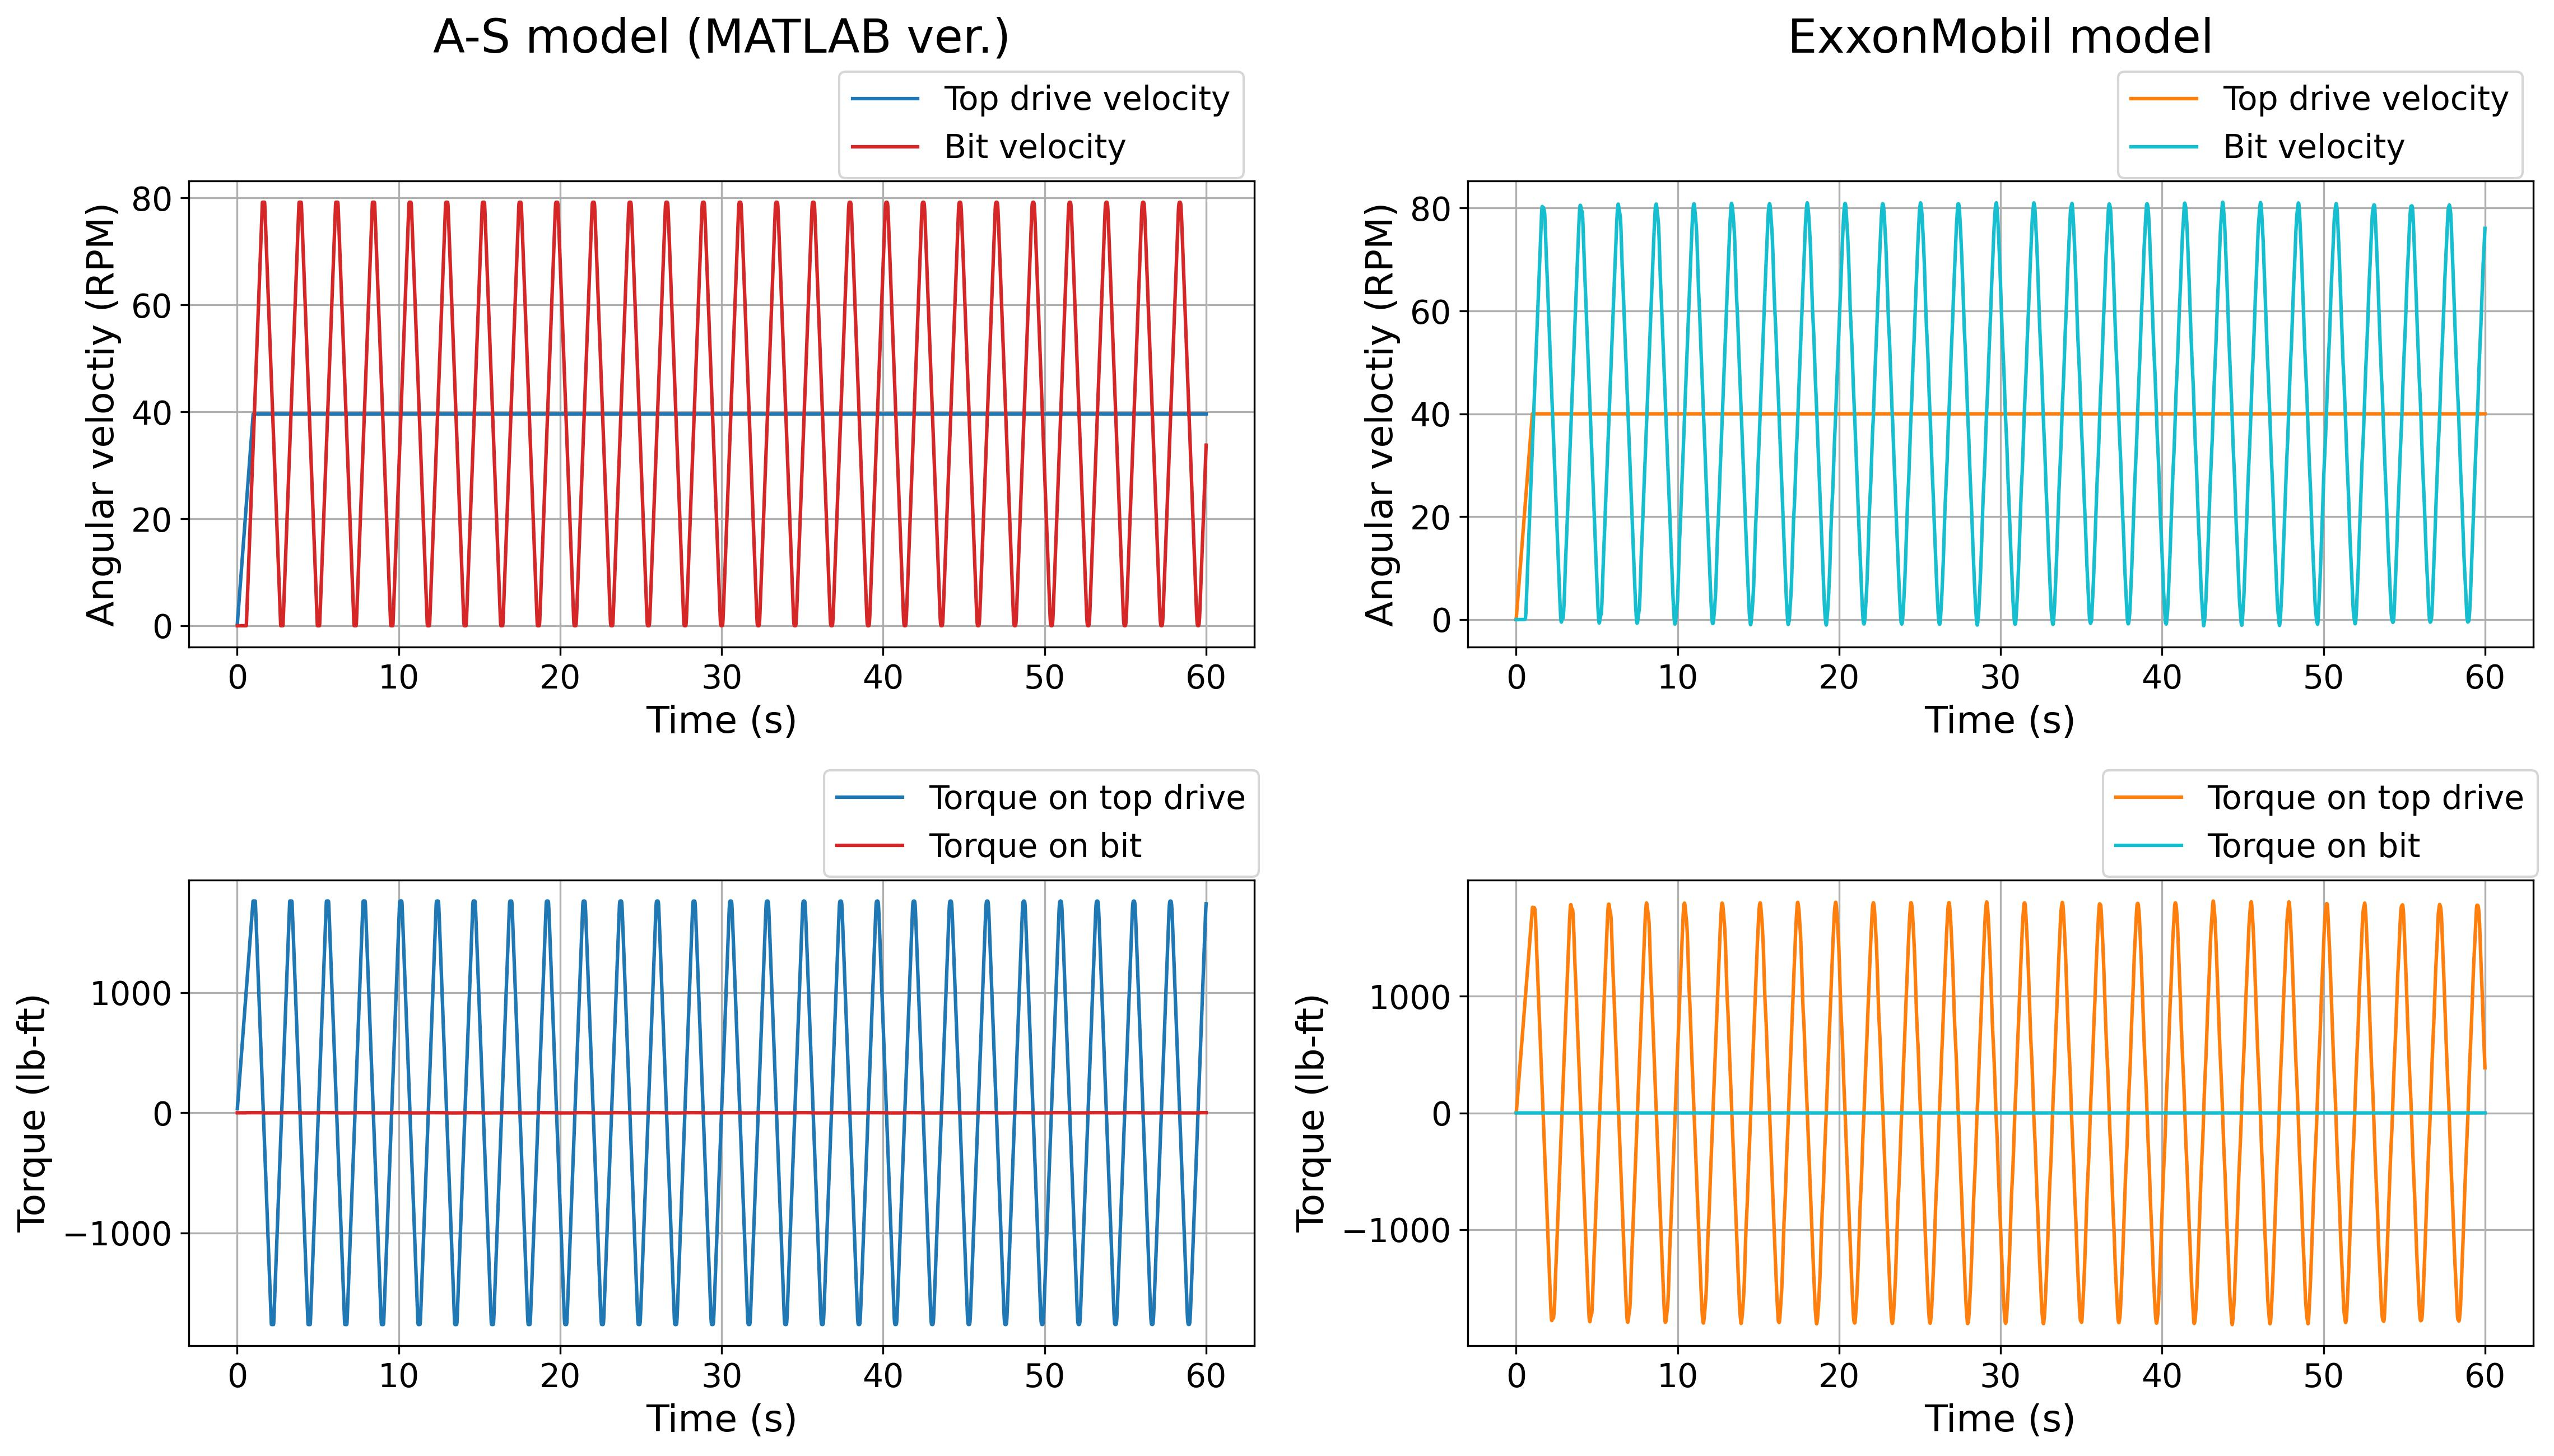
\includegraphics[width=6.5in]{output_figureTestCase1}
  \caption[Angular velocity and torque plots for Test Case 1]{Angular velocity and torque plots for Test Case 1. First and second columns show the results from the A-S model (Matlab ver.) and the ExxonMobil model, respectively.}\label{figure_testcase1}
\end{figure}
\begin{figure}
  \centering
  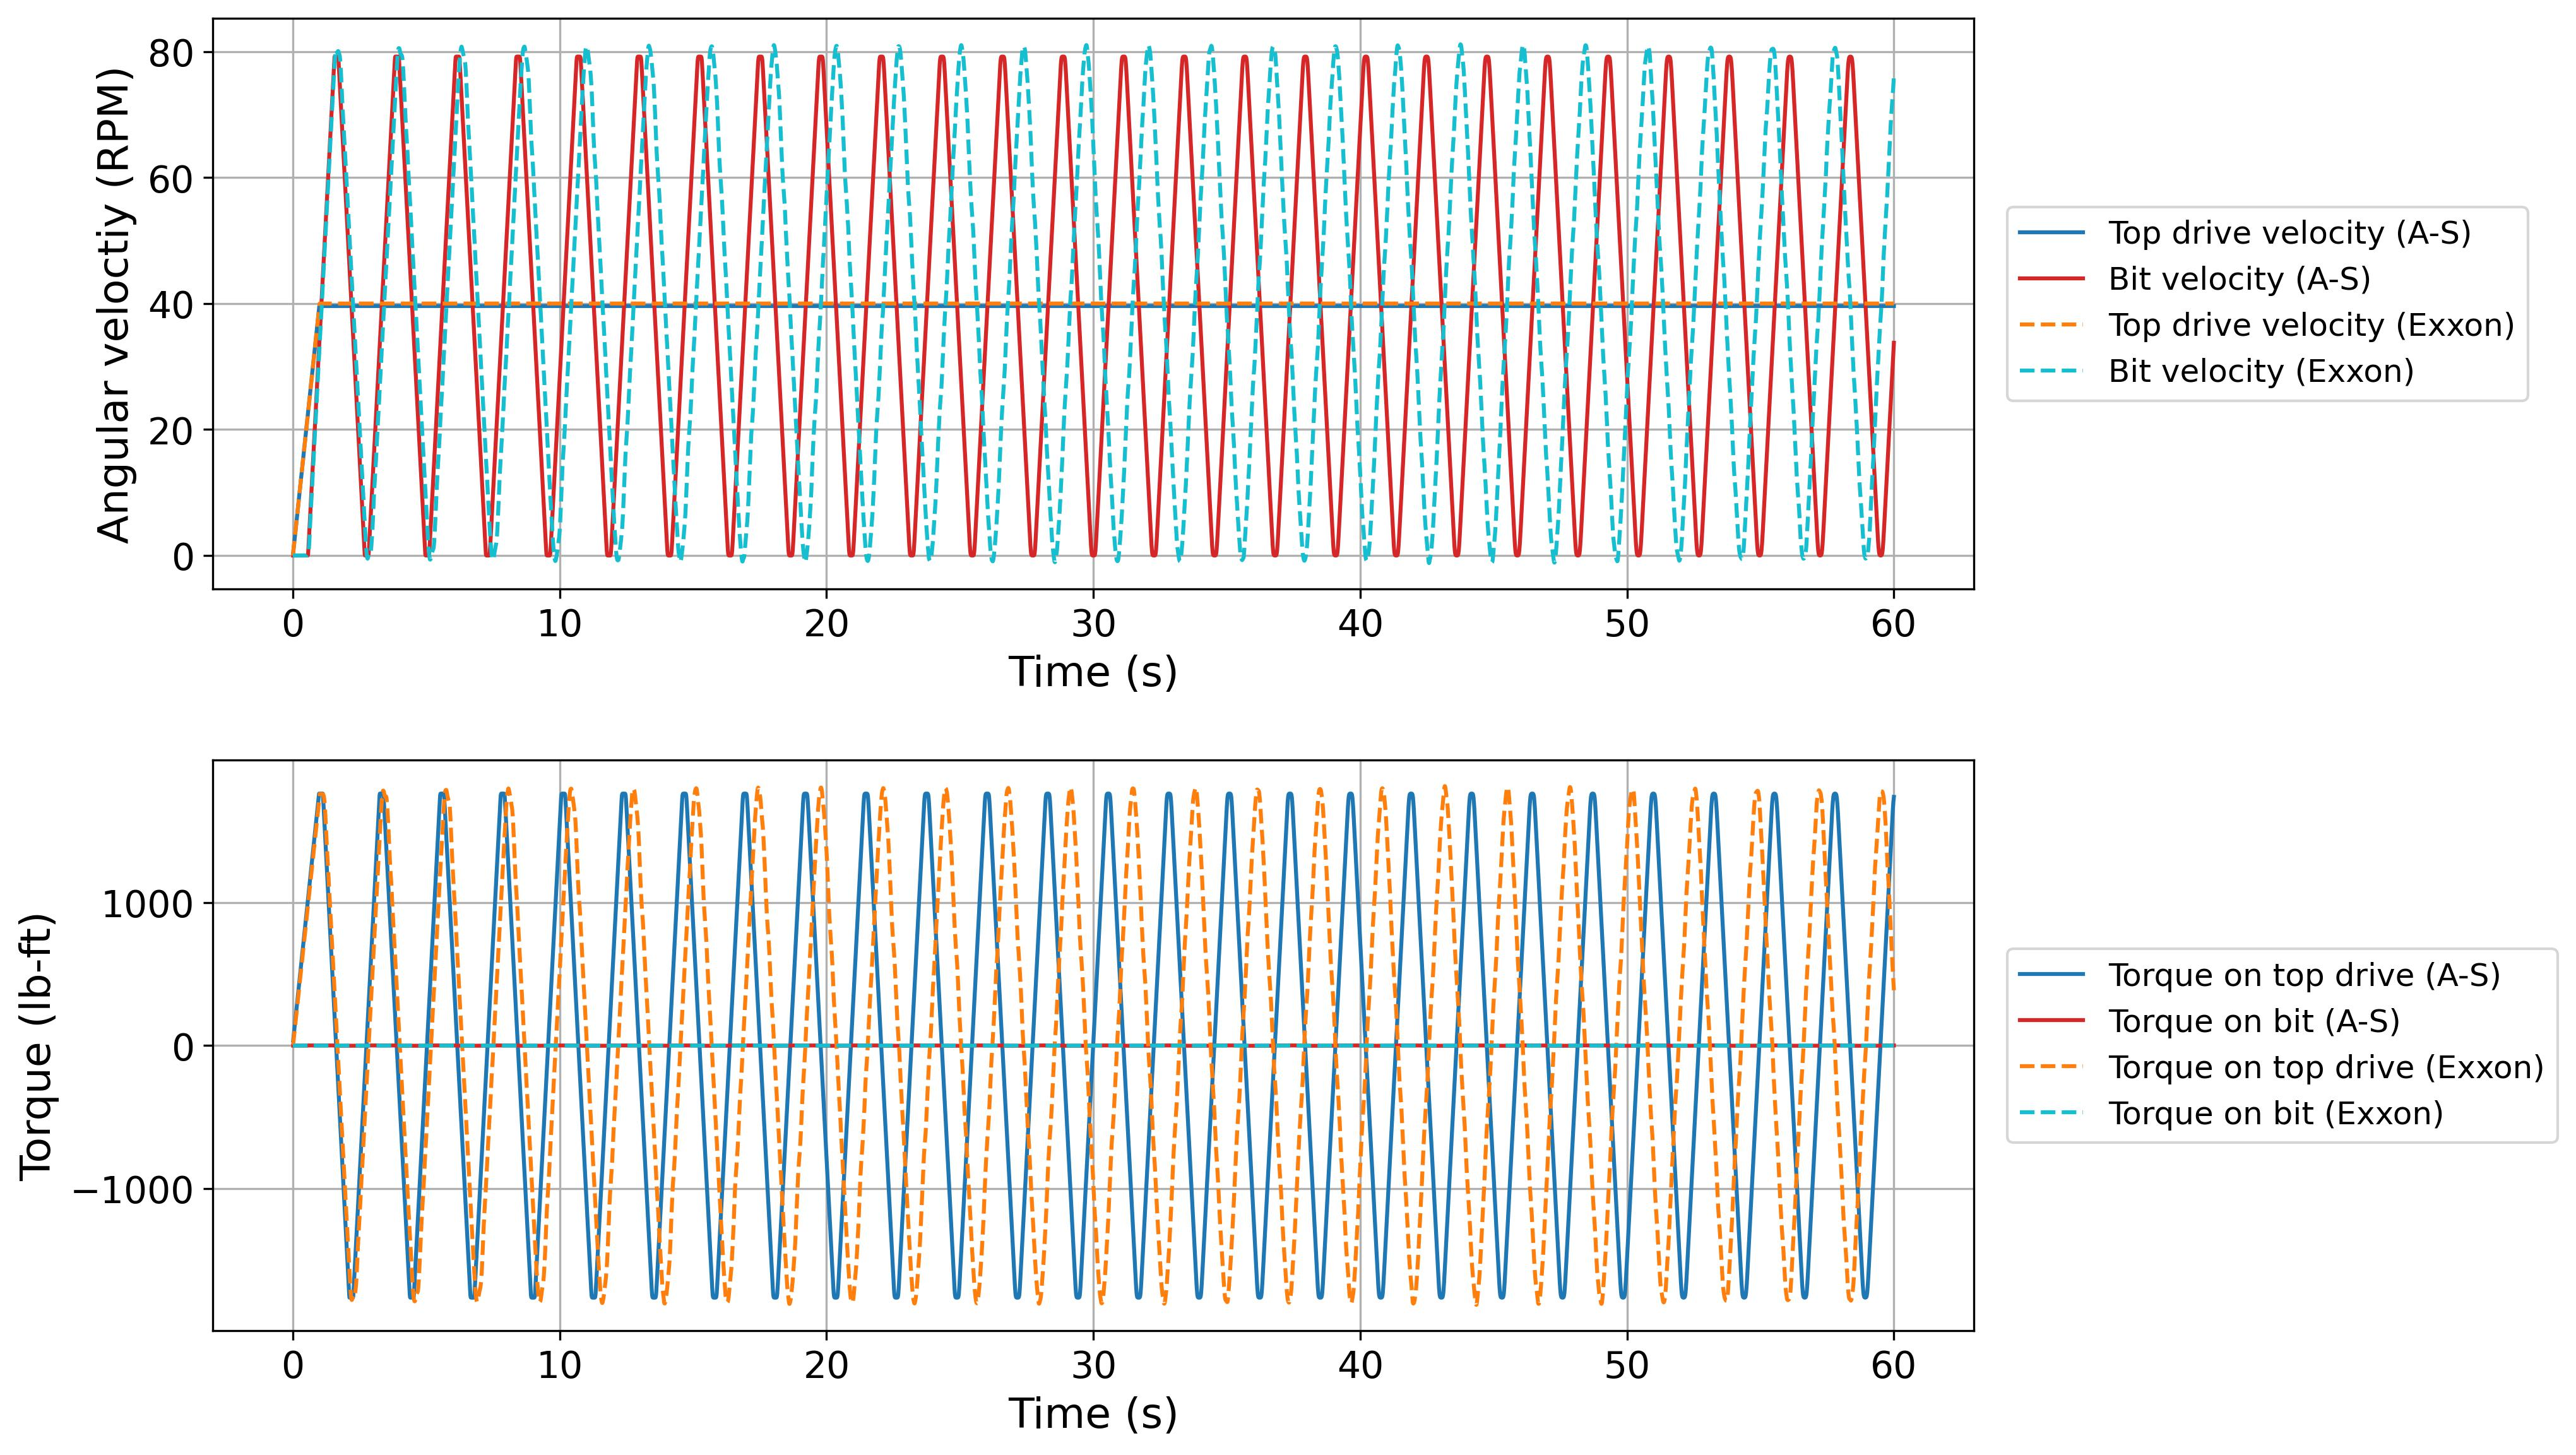
\includegraphics[width=6.5in]{overlapped_figureTestCase1}
  \caption[Angular velocity and torque comparison plots for Test Case 1]{Angular velocity and torque comparison between the A-S model (Matlab ver.) and the ExxonMobil model for Test Case 1. The fundamental vibration frequency are 0.440 $Hz$ from the A-S model and 0.427 $Hz$ from the ExxonMobil model. The difference in frequency is small, but the accumulated effect of this difference caused a phase shift as the simulation continued. Overall, both models matched well, showing similar amplitude of torque and angular velocity of top drive and bit.}\label{figure_testcase1_overlapped}
\end{figure}
\begin{table}
\centering
\begin{tabular}{|c|c|c|}
\hline
\tablecolumnheadervlinesone{} & \tablecolumnheadervlinestwo{A-S Model} & \tablecolumnheadervlinestwo{ExxonMobil Model} \\
\hline
Frequency & 0.440 $Hz$ & 0.427 $Hz$\\
\hline
Maximum bit velocity & 79 $RPM$ & 81 $RPM$ \\
\hline
Maximum top drive torque & 1762 $lb\mbox{-}ft$ & 1814 $lb\mbox{-}ft$ \\
\hline
Computation time & 36 $s$ & 106 $s$\\
\hline
\end{tabular}
\caption[Comparison between the A-S and ExxonMobil models for Test Case 1.]{Comparison between the A-S and ExxonMobil models for Test Case 1.}\label{table_summary_testcase1}
\end{table}

\section{Test Case 2}
Test Case 2 simulates a deviated well scenario without BHA components. In Test Case 2a, both the static and dynamic friction factors are set to 0.5. Test Case 2b uses a static friction factor of 0.5 and a dynamic friction factor of 0.25.

\subsection{Test Case 2a}
The results for Test Case 2a from each model are depicted in \figurename~\ref{figure_testcase2_1}. Similar to Test Case 1, both models are well matched with fundamental vibration frequencies of 0.283 $Hz$ and 0.272 $Hz$ for the A-S model and the ExxonMobil model, respectively. The maximum bit velocity was at 78 $RPM$ for the A-S model and 79 $RPM$ for the ExxonMobil model, while the maximum torque on the top drive was predicted as 6643 $lb\mbox{-}ft$ for the A-S model and 6891 $lb\mbox{-}ft$ for the ExxonMobil model. \figurename~\ref{figure_testcase2_1_overlapped} illustrates the comparison of the results from two different models and the features are summarized in \tablename~\ref{table_summary_testcase2a}.
\begin{figure}
  \centering
  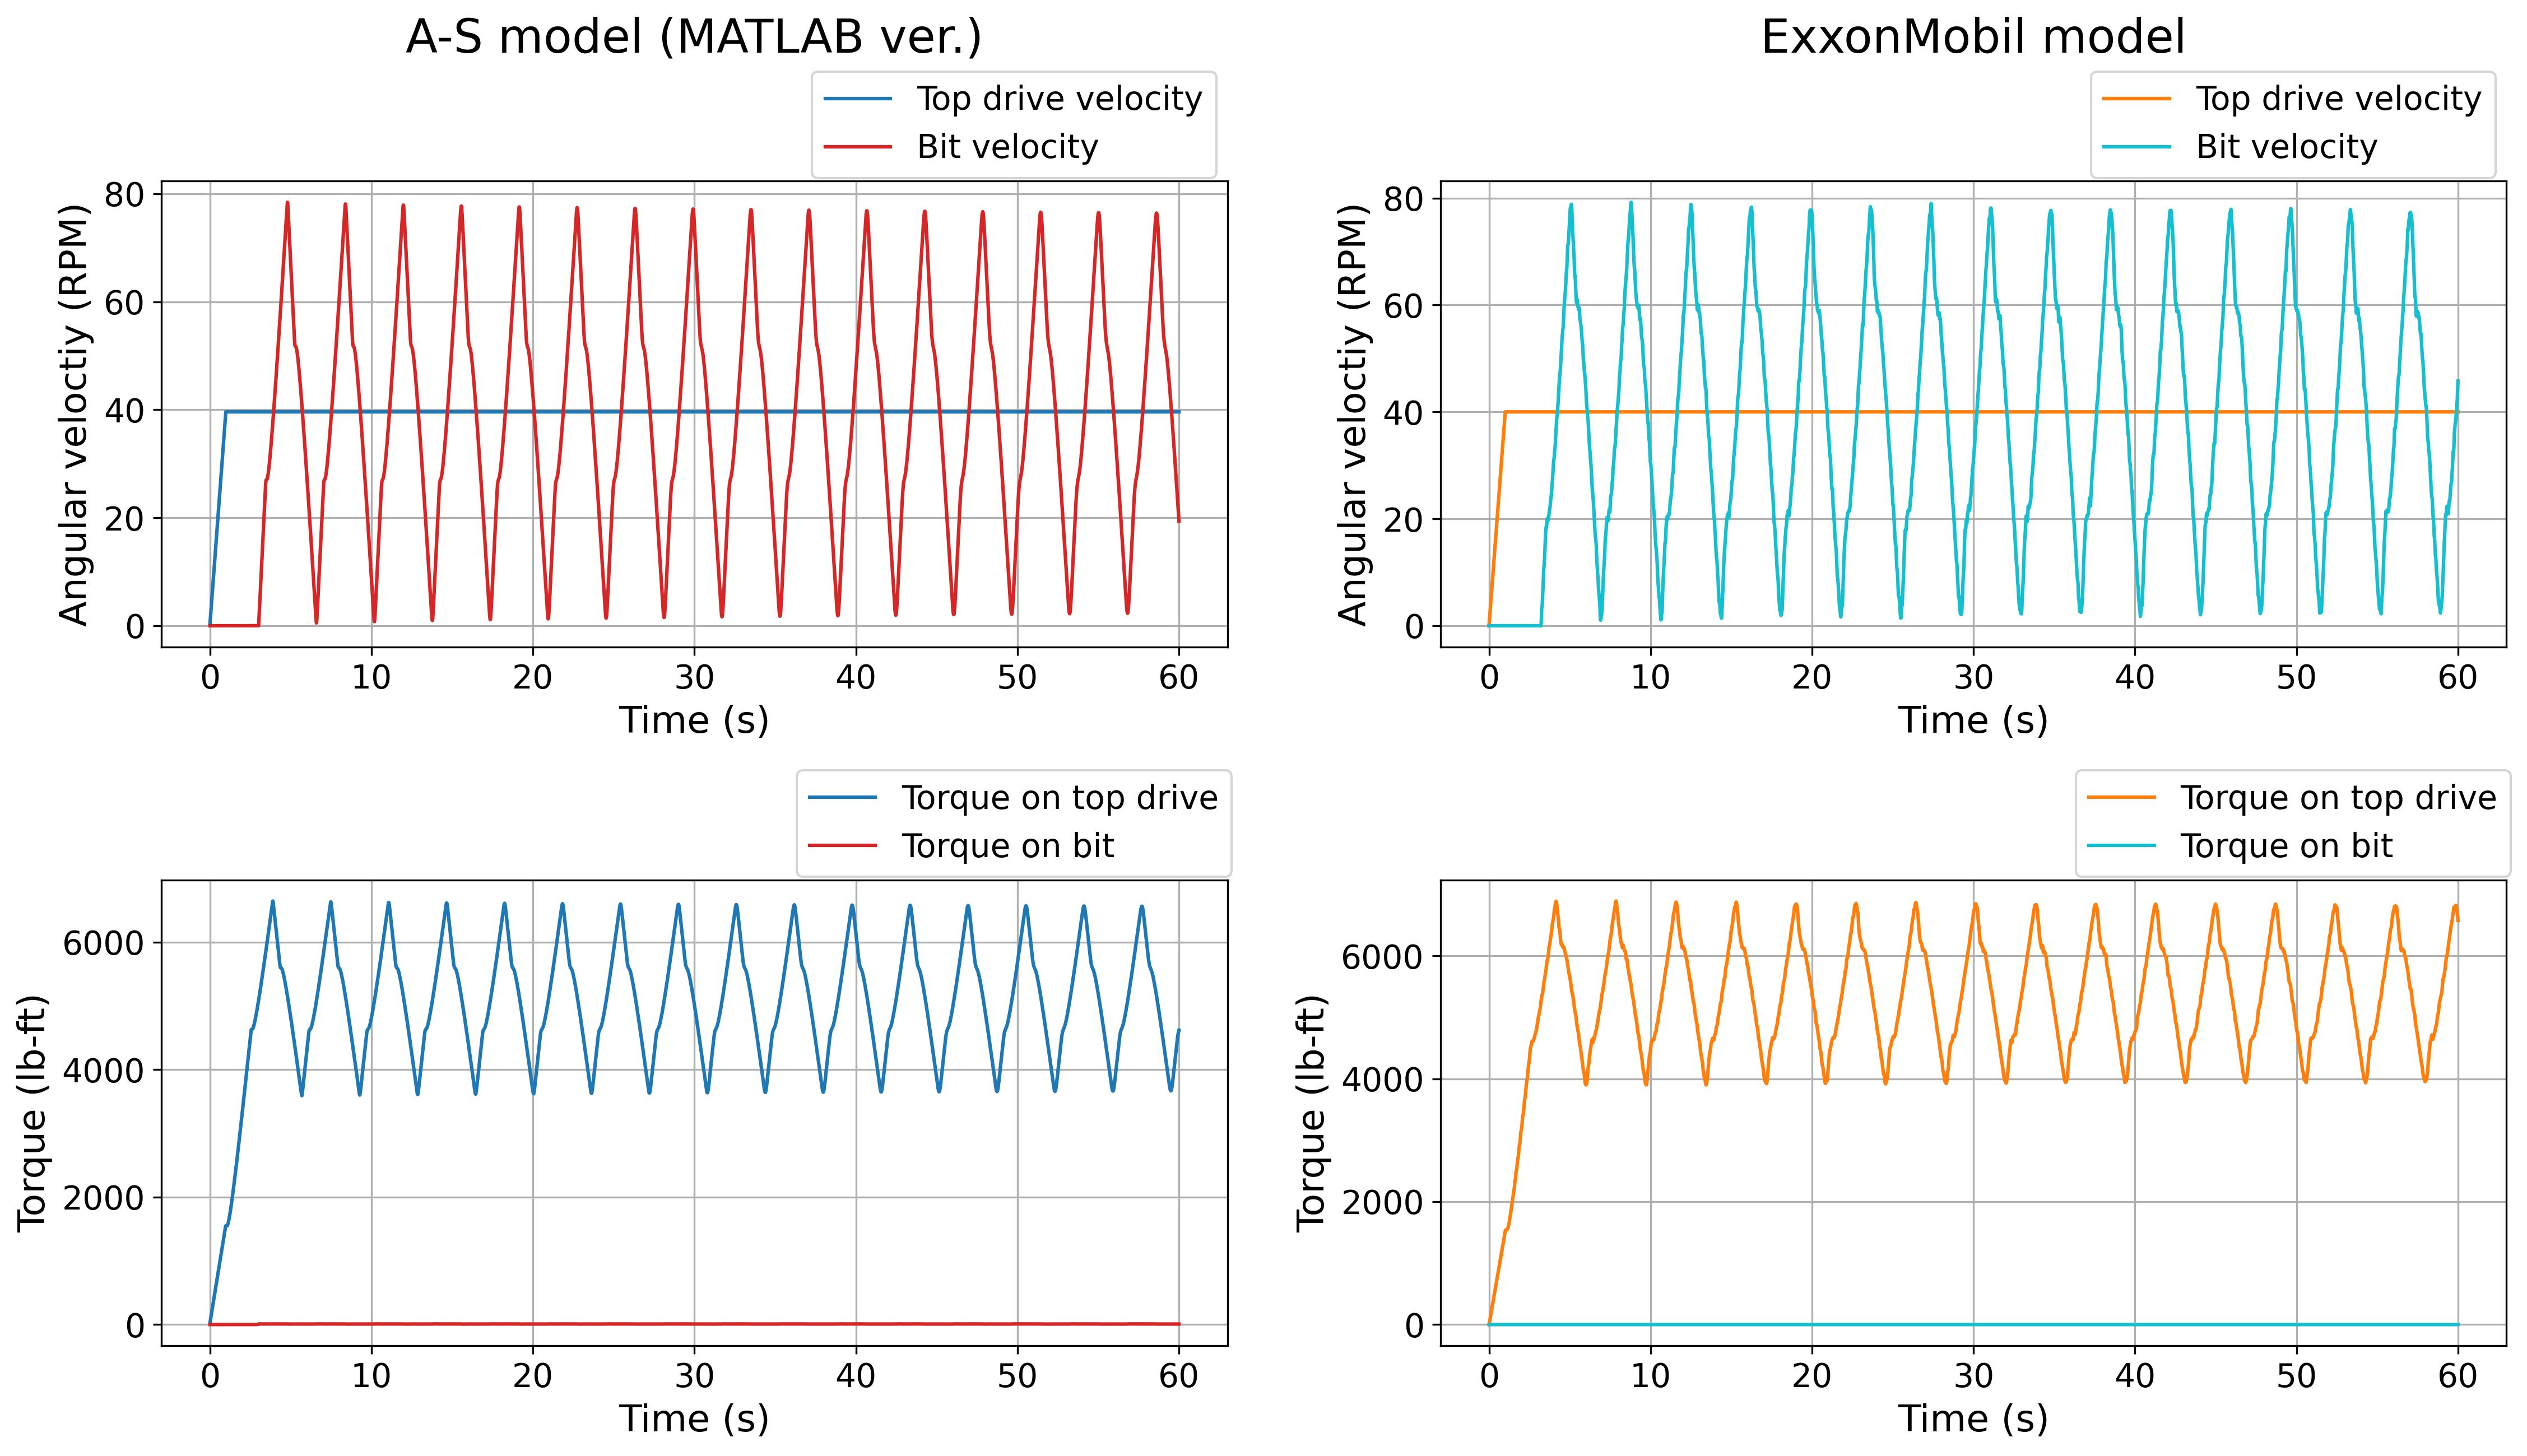
\includegraphics[width=6.5in]{output_figureTestCase2_1}
  \caption[Angular velocity and torque plots for Test Case 2a]{Angular velocity and torque plots for Test Case 2a. First and second columns show the results from the A-S model (Matlab ver.) and the ExxonMobil model, respectively.}\label{figure_testcase2_1}
\end{figure}

\begin{figure}
  \centering
  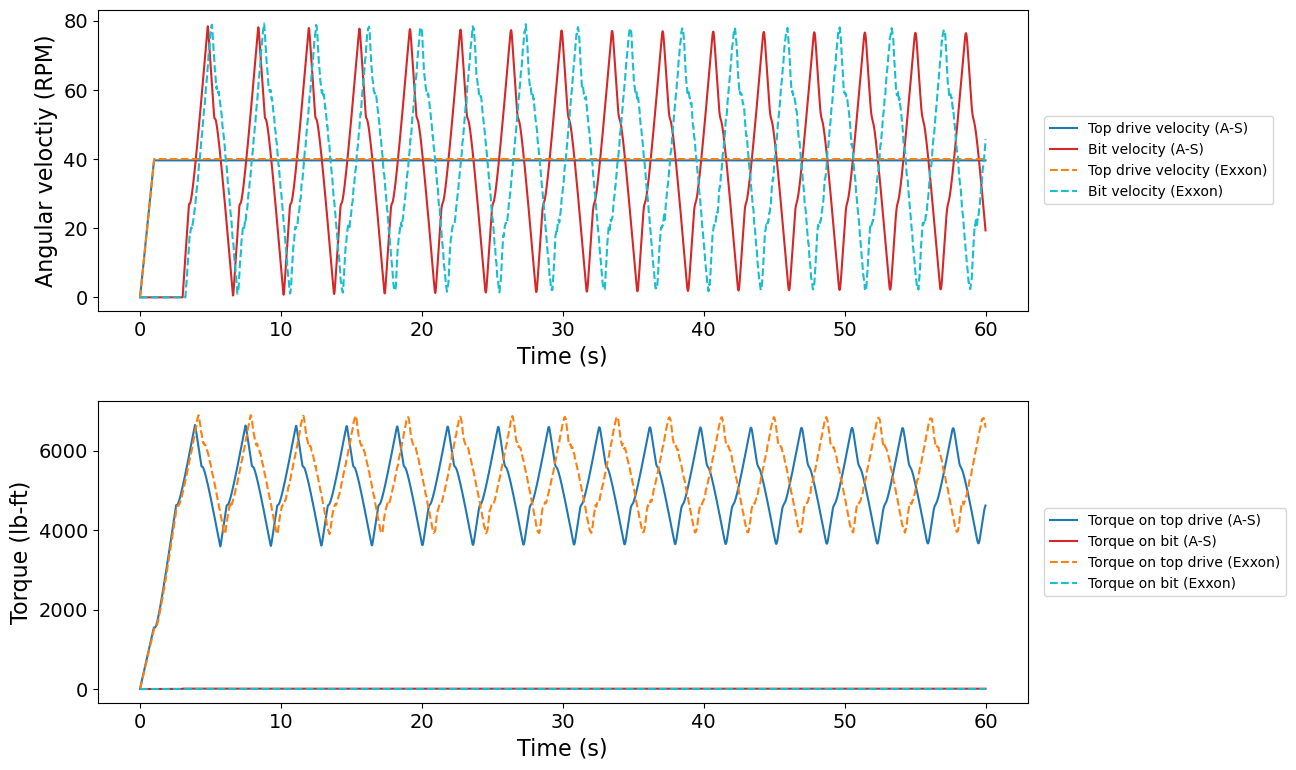
\includegraphics[width=6.5in]{overlapped_figureTestCase2_1}
  \caption[Angular velocity and torque comparison plots for Test Case 2a]{Angular velocity and torque comparison between the results from the A-S model (Matlab ver.) and the ExxonMobil model for Test Case 2a. The fundamental vibration frequency are 0.283 $Hz$ from the A-S model and 0.272 $Hz$ from the ExxonMobil model. The difference in frequency is small but the accumulated effect of this differences caused the phase shift during 60 seconds. Overall, both models matched well showing similar amplitude of torque and angular velocity of top drive and bit.}\label{figure_testcase2_1_overlapped}
\end{figure}
\begin{table}
\centering
\begin{tabular}{|c|c|c|}
\hline
\tablecolumnheadervlinesone{} & \tablecolumnheadervlinestwo{A-S Model} & \tablecolumnheadervlinestwo{ExxonMobil Model} \\
\hline
Frequency & 0.283 $Hz$ & 0.272 $Hz$\\
\hline
Maximum bit velocity & 78 $RPM$ & 79 $RPM$ \\
\hline
Maximum top drive torque & 6643 $lb\mbox{-}ft$ & 6891 $lb\mbox{-}ft$ \\
\hline
Computation time & 25 $s$ & 117 $s$\\
\hline
\end{tabular}
\caption[Comparison between the A-S and ExxonMobil models for Test Case 2a]{Comparison between the A-S model and ExxonMobil model for Test Case 2a.}\label{table_summary_testcase2a}
\end{table}


\subsection{Test Case 2b}
The results for Test Case 2b from each model are depicted in \figurename~\ref{figure_testcase2_2}. The stick-slip behavior during drilling was observed in both models. Both models showed transient behavior until 40 seconds and showed almost consistent patterns of vibration after 40 seconds. The period of the stick phase steadily increased from the beginning and reached about 1.75 seconds for the A-S model and 1.78 seconds for the ExxonMobil model. This stick-slip event was caused by friction in the deviated well.  The effect of the dynamic friction factor---the only variable changed---can be seen by comparing Test Cases 2a and 2b. Both models showed a spike in bit angular velocity which goes below zero. This was not investigated and it is recommended that the cause be explored in future studies. Both models showed very similar responses, especially in the transient duration (before 40 seconds).

The fundamental frequencies of the vibration were 0.280 $Hz$ and 0.269 $Hz$ for the A-S model and the ExxonMobil model, respectively.  These are similar to Test Case 2a. The maximum bit velocity was at 107 $RPM$ for the A-S model and 116 $RPM$ for the ExxonMobil model. The maximum torque on the top drive was predicted as 5185 $lb\mbox{-}ft$ for the A-S model and 5540 $lb\mbox{-}ft$ for the ExxonMobil model and occurred at the first cycle for both cases. \figurename~\ref{figure_testcase2_2_overlapped} illustrates the comparison of the results from two different models during 60 seconds of modeling. Relatively similar behavior can be seen from the comparison and also the effect of the phase shift was observed. The comparison of the features from each model's result is shown in \tablename~\ref{table_summary_testcase2b}.

\begin{figure}
  \centering
  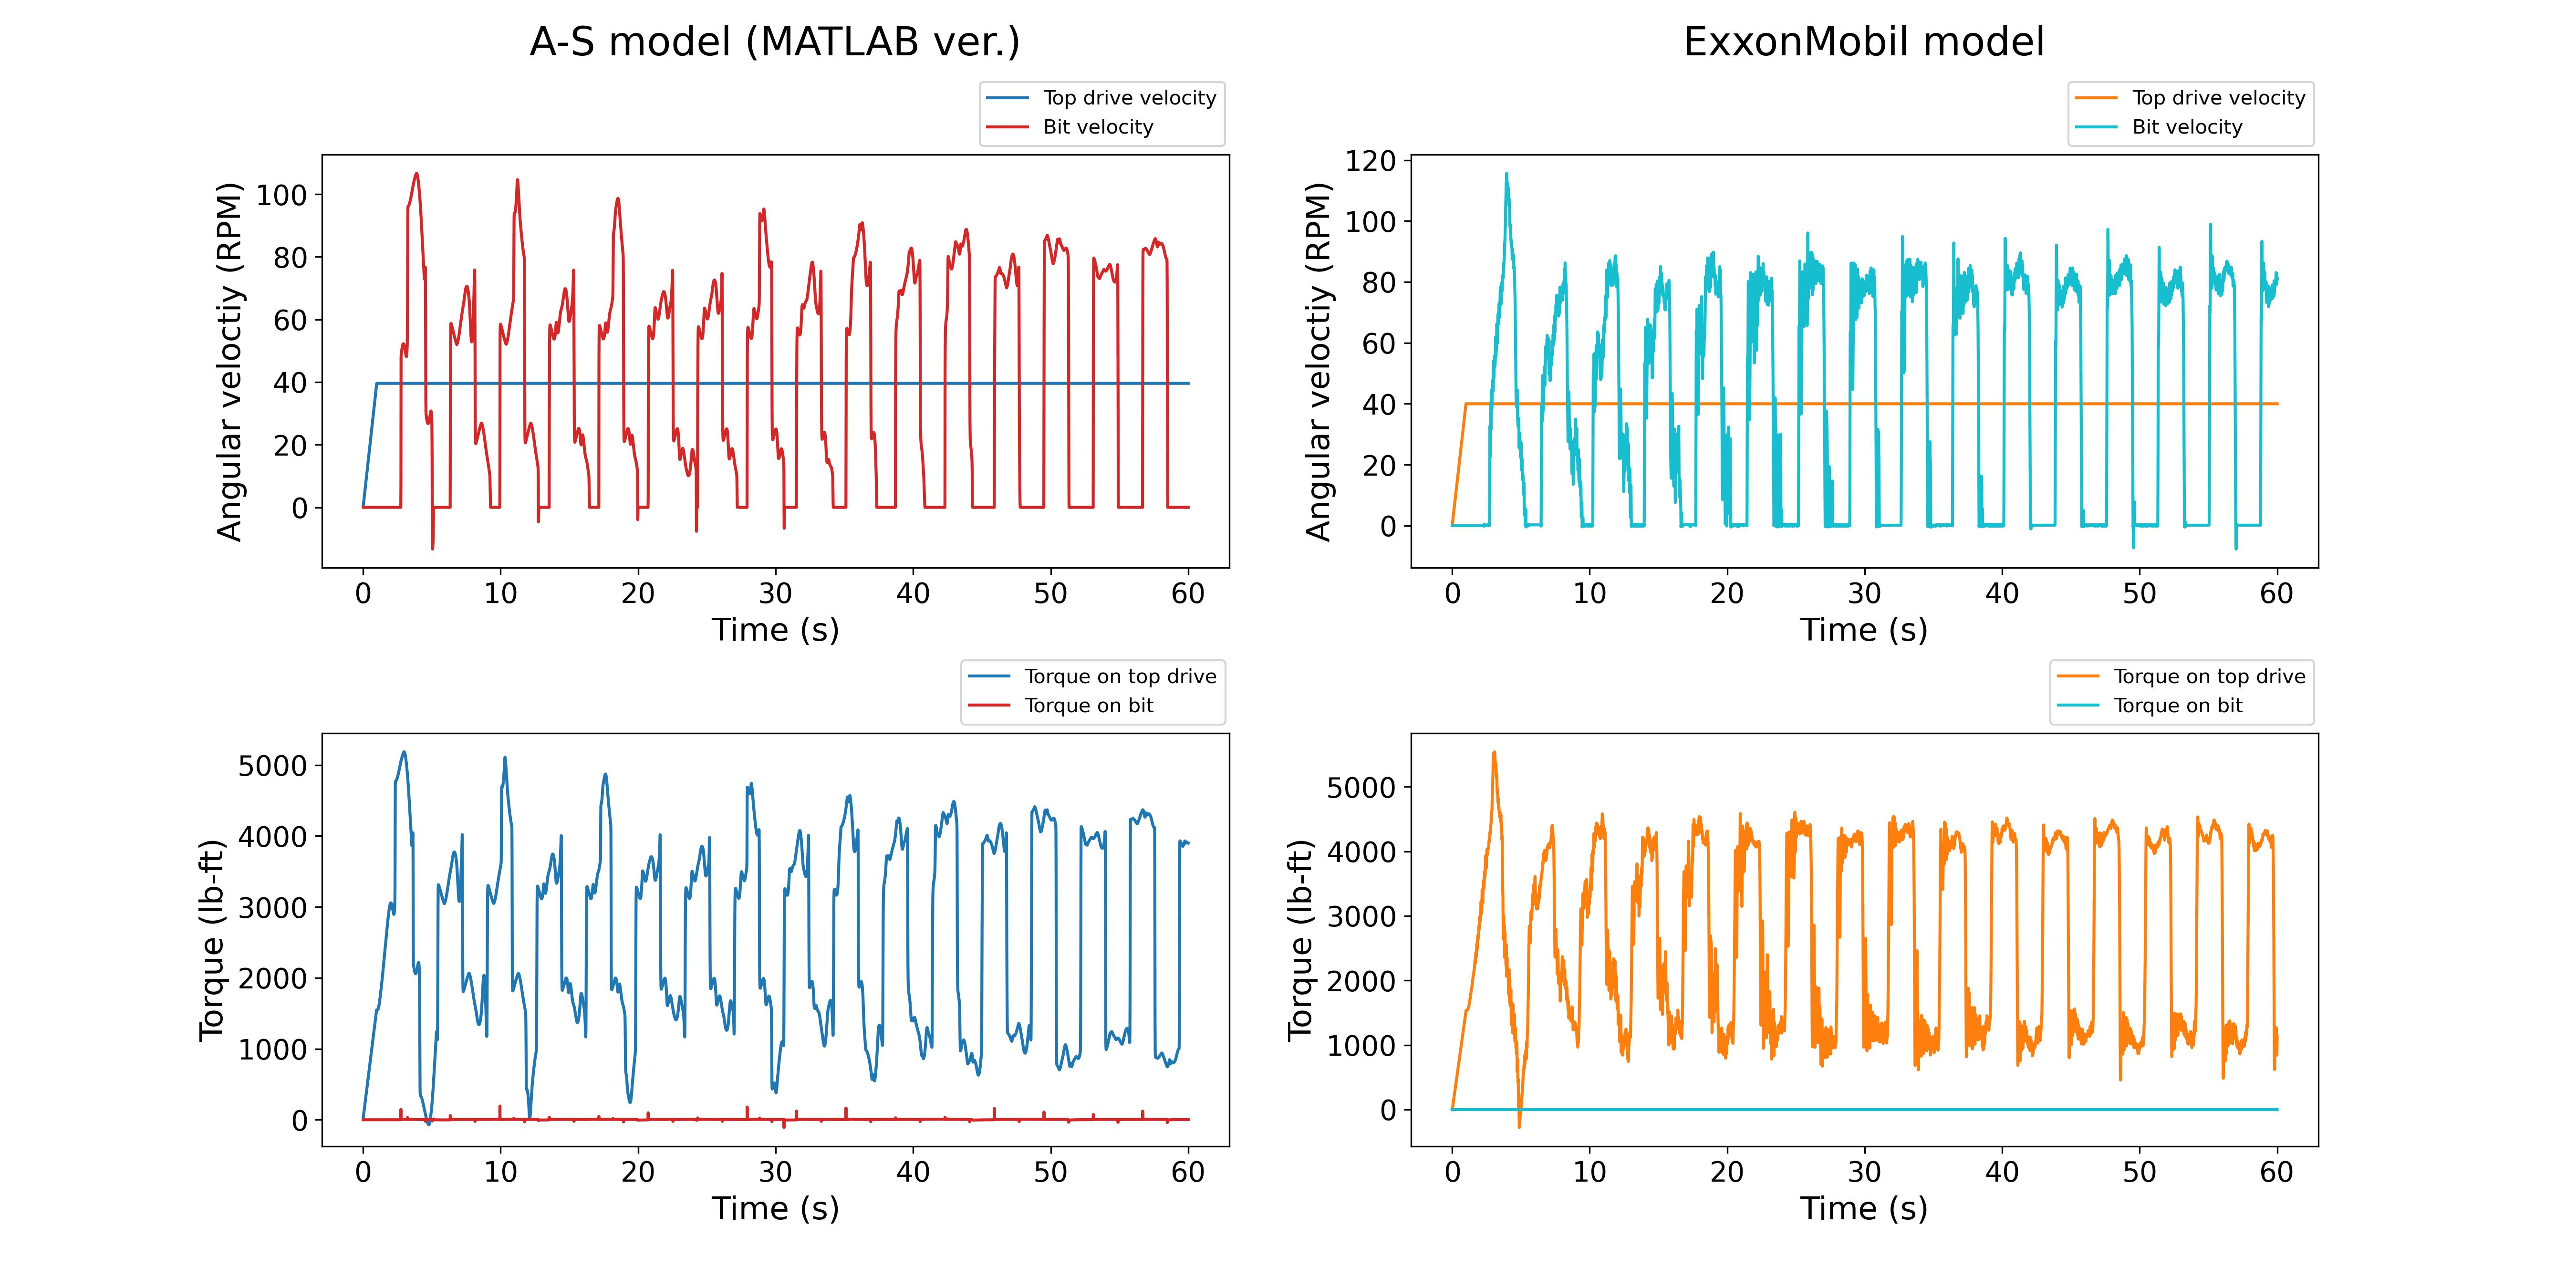
\includegraphics[width=6.5in]{output_figureTestCase2_2}
  \caption[Angular velocity and torque plots for Test Case 2b]{Angular velocity and torque plots for Test Case 2b. First and second columns show the results from the A-S model (Matlab ver.) and the ExxonMobil model, respectively.}\label{figure_testcase2_2}
\end{figure}

\begin{figure}
  \centering
  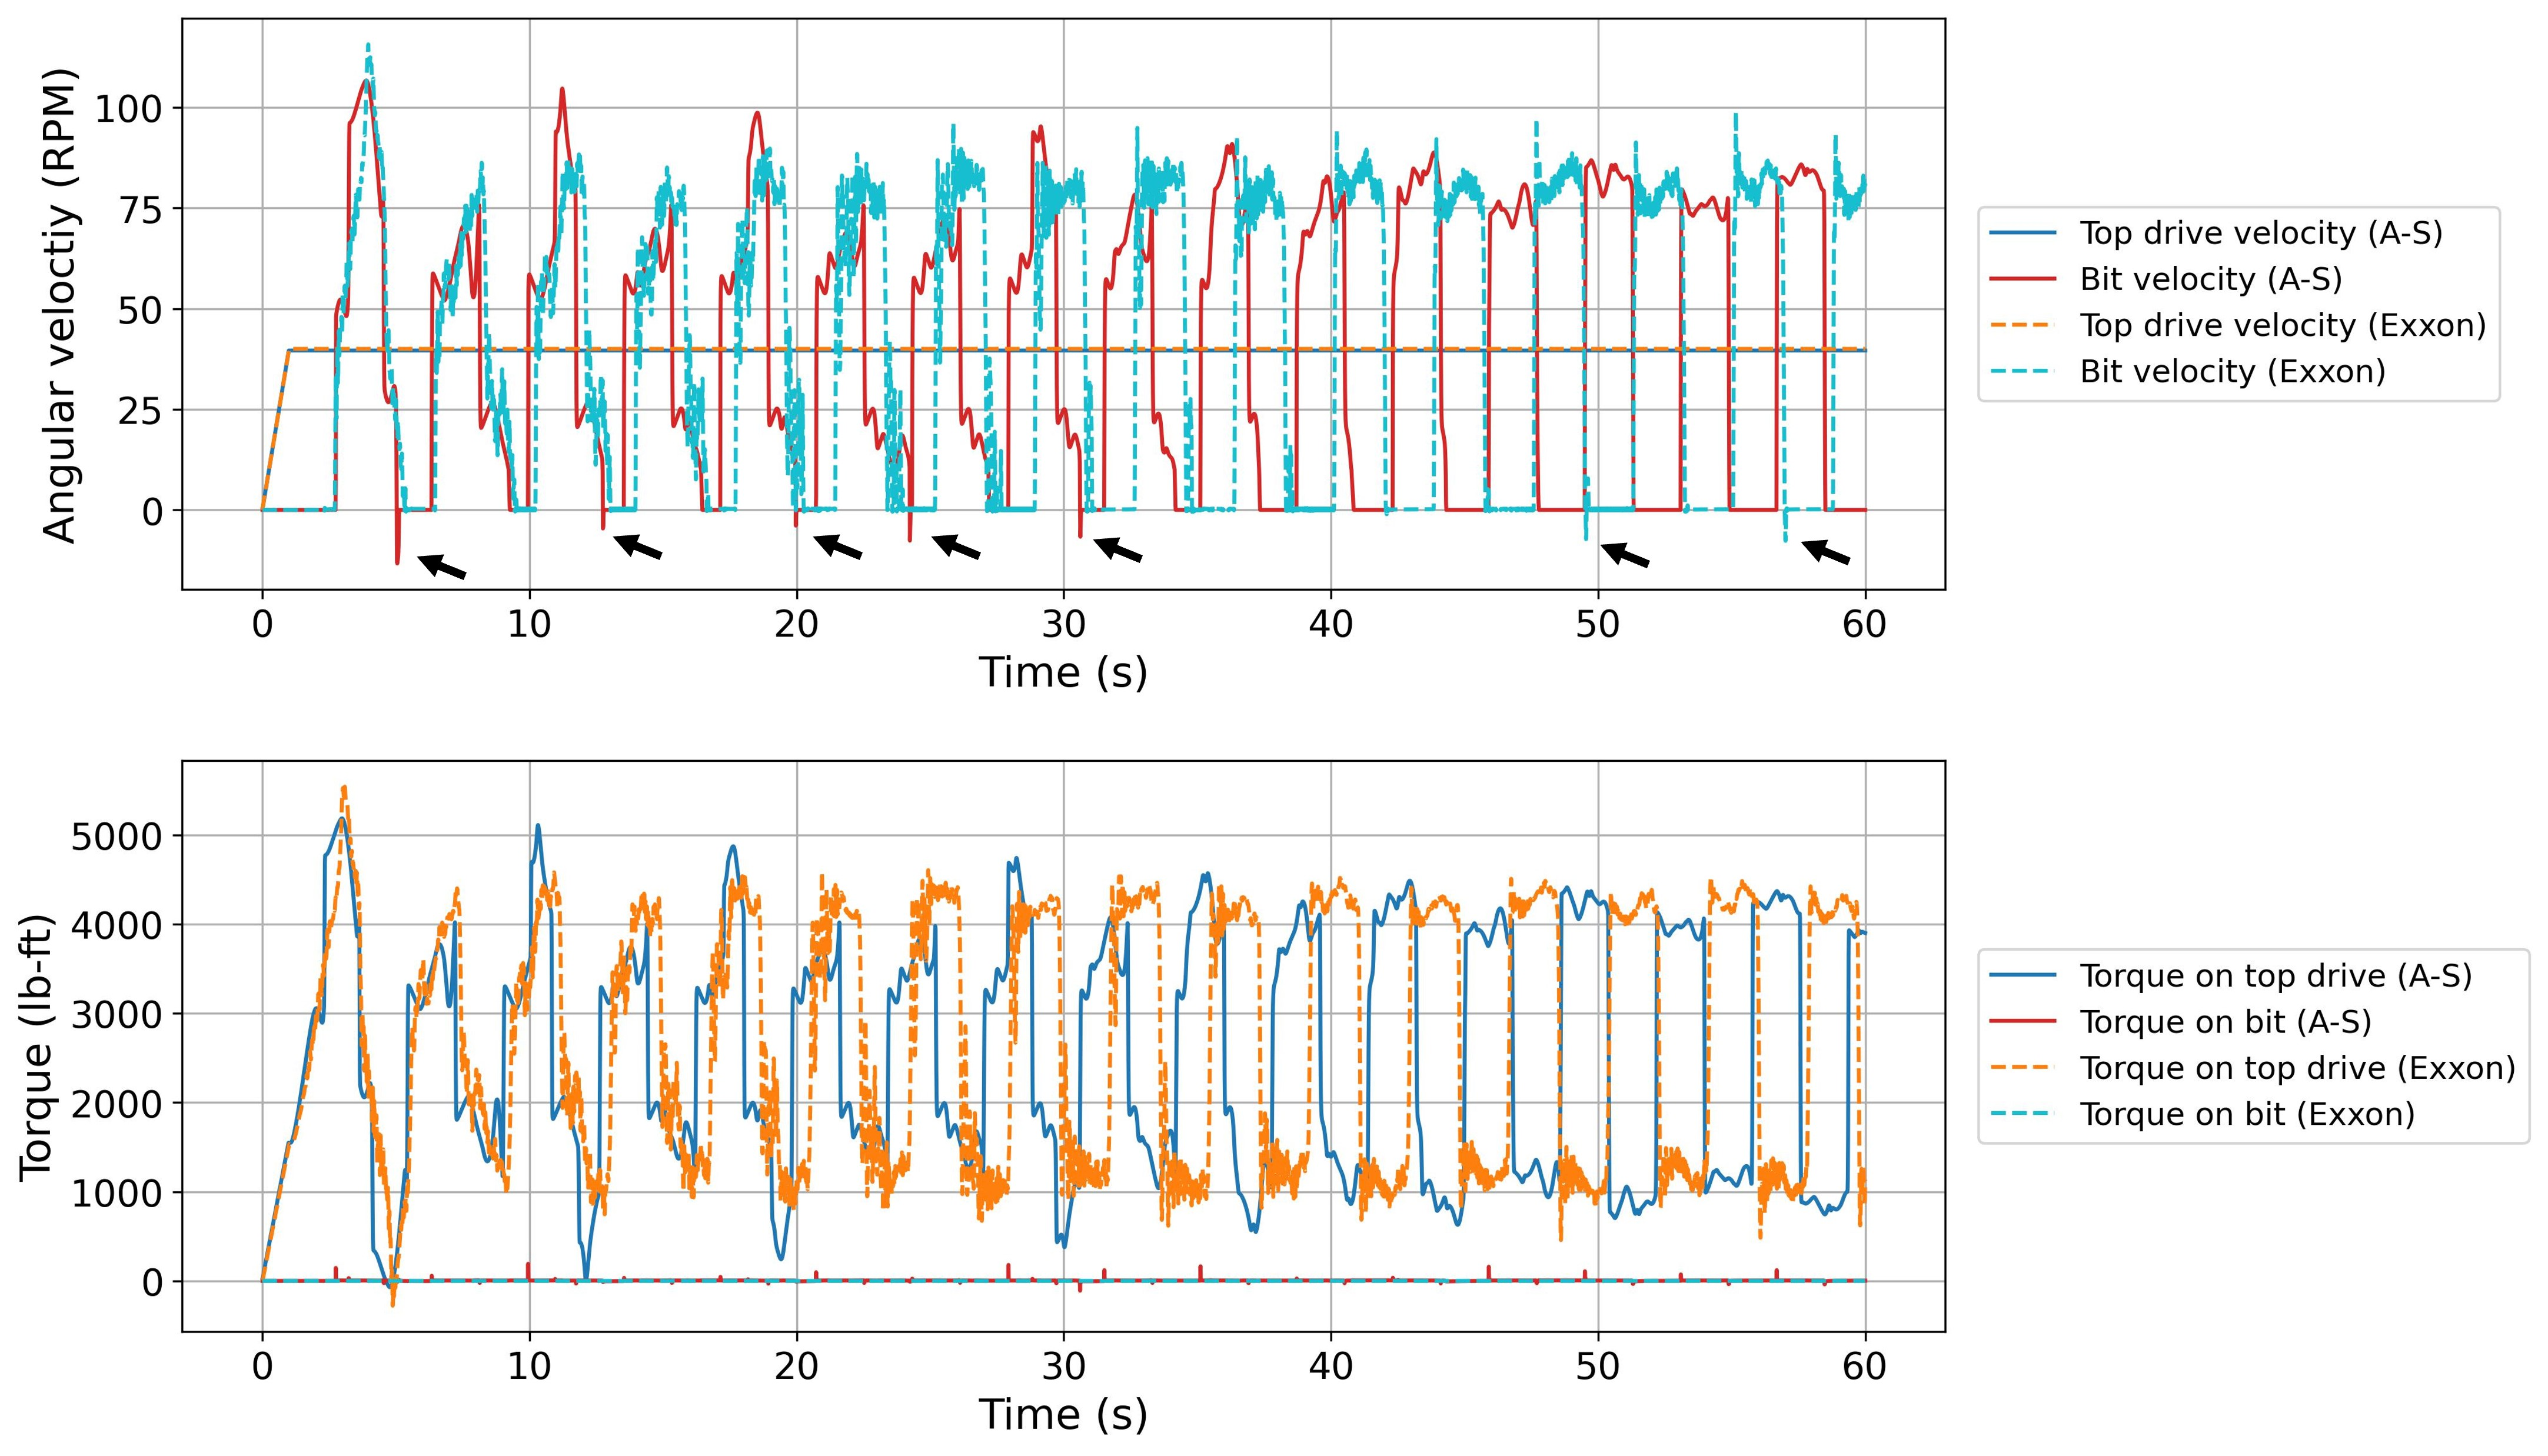
\includegraphics[width=6.5in]{overlapped_figureTestCase2_2_arrow}
  \caption[Angular velocity and torque comparison plots for Test Case 2b]{Angular velocity and torque comparison of the results from the A-S model (Matlab ver.) and the ExxonMobil model for Test Case 2b. Both models demonstrated stick-slip. The fundamental vibration frequencies are 0.280 $Hz$ for the A-S model and 0.269 $Hz$ for the ExxonMobil model. The difference in frequency is small, but the accumulated effect of these differences caused the phase shift during 60 seconds. Overall, both models matched well. The transient phase (before 40 seconds) showed similar vibration patterns for both models. Both models predicted a similar standstill duration of 1.6-1.8 seconds during the stick phase (after 40 seconds). The spikes in bit angular velocity ($<$ 0) were observed from both models, which are pointed out by black arrows.}\label{figure_testcase2_2_overlapped}
\end{figure}
\begin{table}
\centering
\begin{tabular}{|c|c|c|}
\hline
\tablecolumnheadervlinesone{} & \tablecolumnheadervlinestwo{A-S Model} & \tablecolumnheadervlinestwo{ExxonMobil Model} \\
\hline
Frequency & 0.280 $Hz$ & 0.269 $Hz$\\
\hline
Maximum bit velocity & 106 $RPM$ & 115 $RPM$ \\
\hline
Maximum top drive torque & 5184 $lb\mbox{-}ft$ & 5539 $lb\mbox{-}ft$ \\
\hline
Computation time & 25 $s$ & 116 $s$\\
\hline
\end{tabular}
\caption[Comparison between the A-S and ExxonMobil models for Test Case 2b]{Comparison between the A-S and ExxonMobil models for Test Case 2b.}\label{table_summary_testcase2b}
\end{table}
\section{Test Case 3}
 Test Case 3 represents the scenario of a vertical well with BHA components. The results show similarities with Test Case 1 (vertical well without BHA components), but fluctuations in the peak values of the vibration for both bit angular velocity and top drive torque were observed. Specifically, the peak value decreases until 80 seconds and then starts to increase again, returning to the peak value at 120 seconds. \figurename{}s~\ref{figure_testcase3} and~\ref{figure_testcase3_overlapped} illustrate the results for each model and comparisons for Test Case 3. \figurename~\ref{figure_testcase3_overlapped} shows the simulation results for a longer time length (120 seconds) to clearly show the change in the peak values. The results of each model are summarized in \tablename~\ref{table_summary_testcase3}

Compared to Test Case 1 (without BHA components), the fundamental vibration frequencies in Test Case 3 were slightly decreased to 0.420 $Hz$ for the A-S model and 0.408 $Hz$ for the ExxonMobil model. Conversely, the bit velocity and torque on the top drive increased. The maximum bit velocity was 80 $RPM$ for the A-S model and 81 $RPM$ for the ExxonMobil model, while the torque on the top drive was predicted as 1844 $lb\mbox{-}ft$ for the A-S model and 1841 $lb\mbox{-}ft$ for the ExxonMobil model.

\begin{figure}
  \centering
  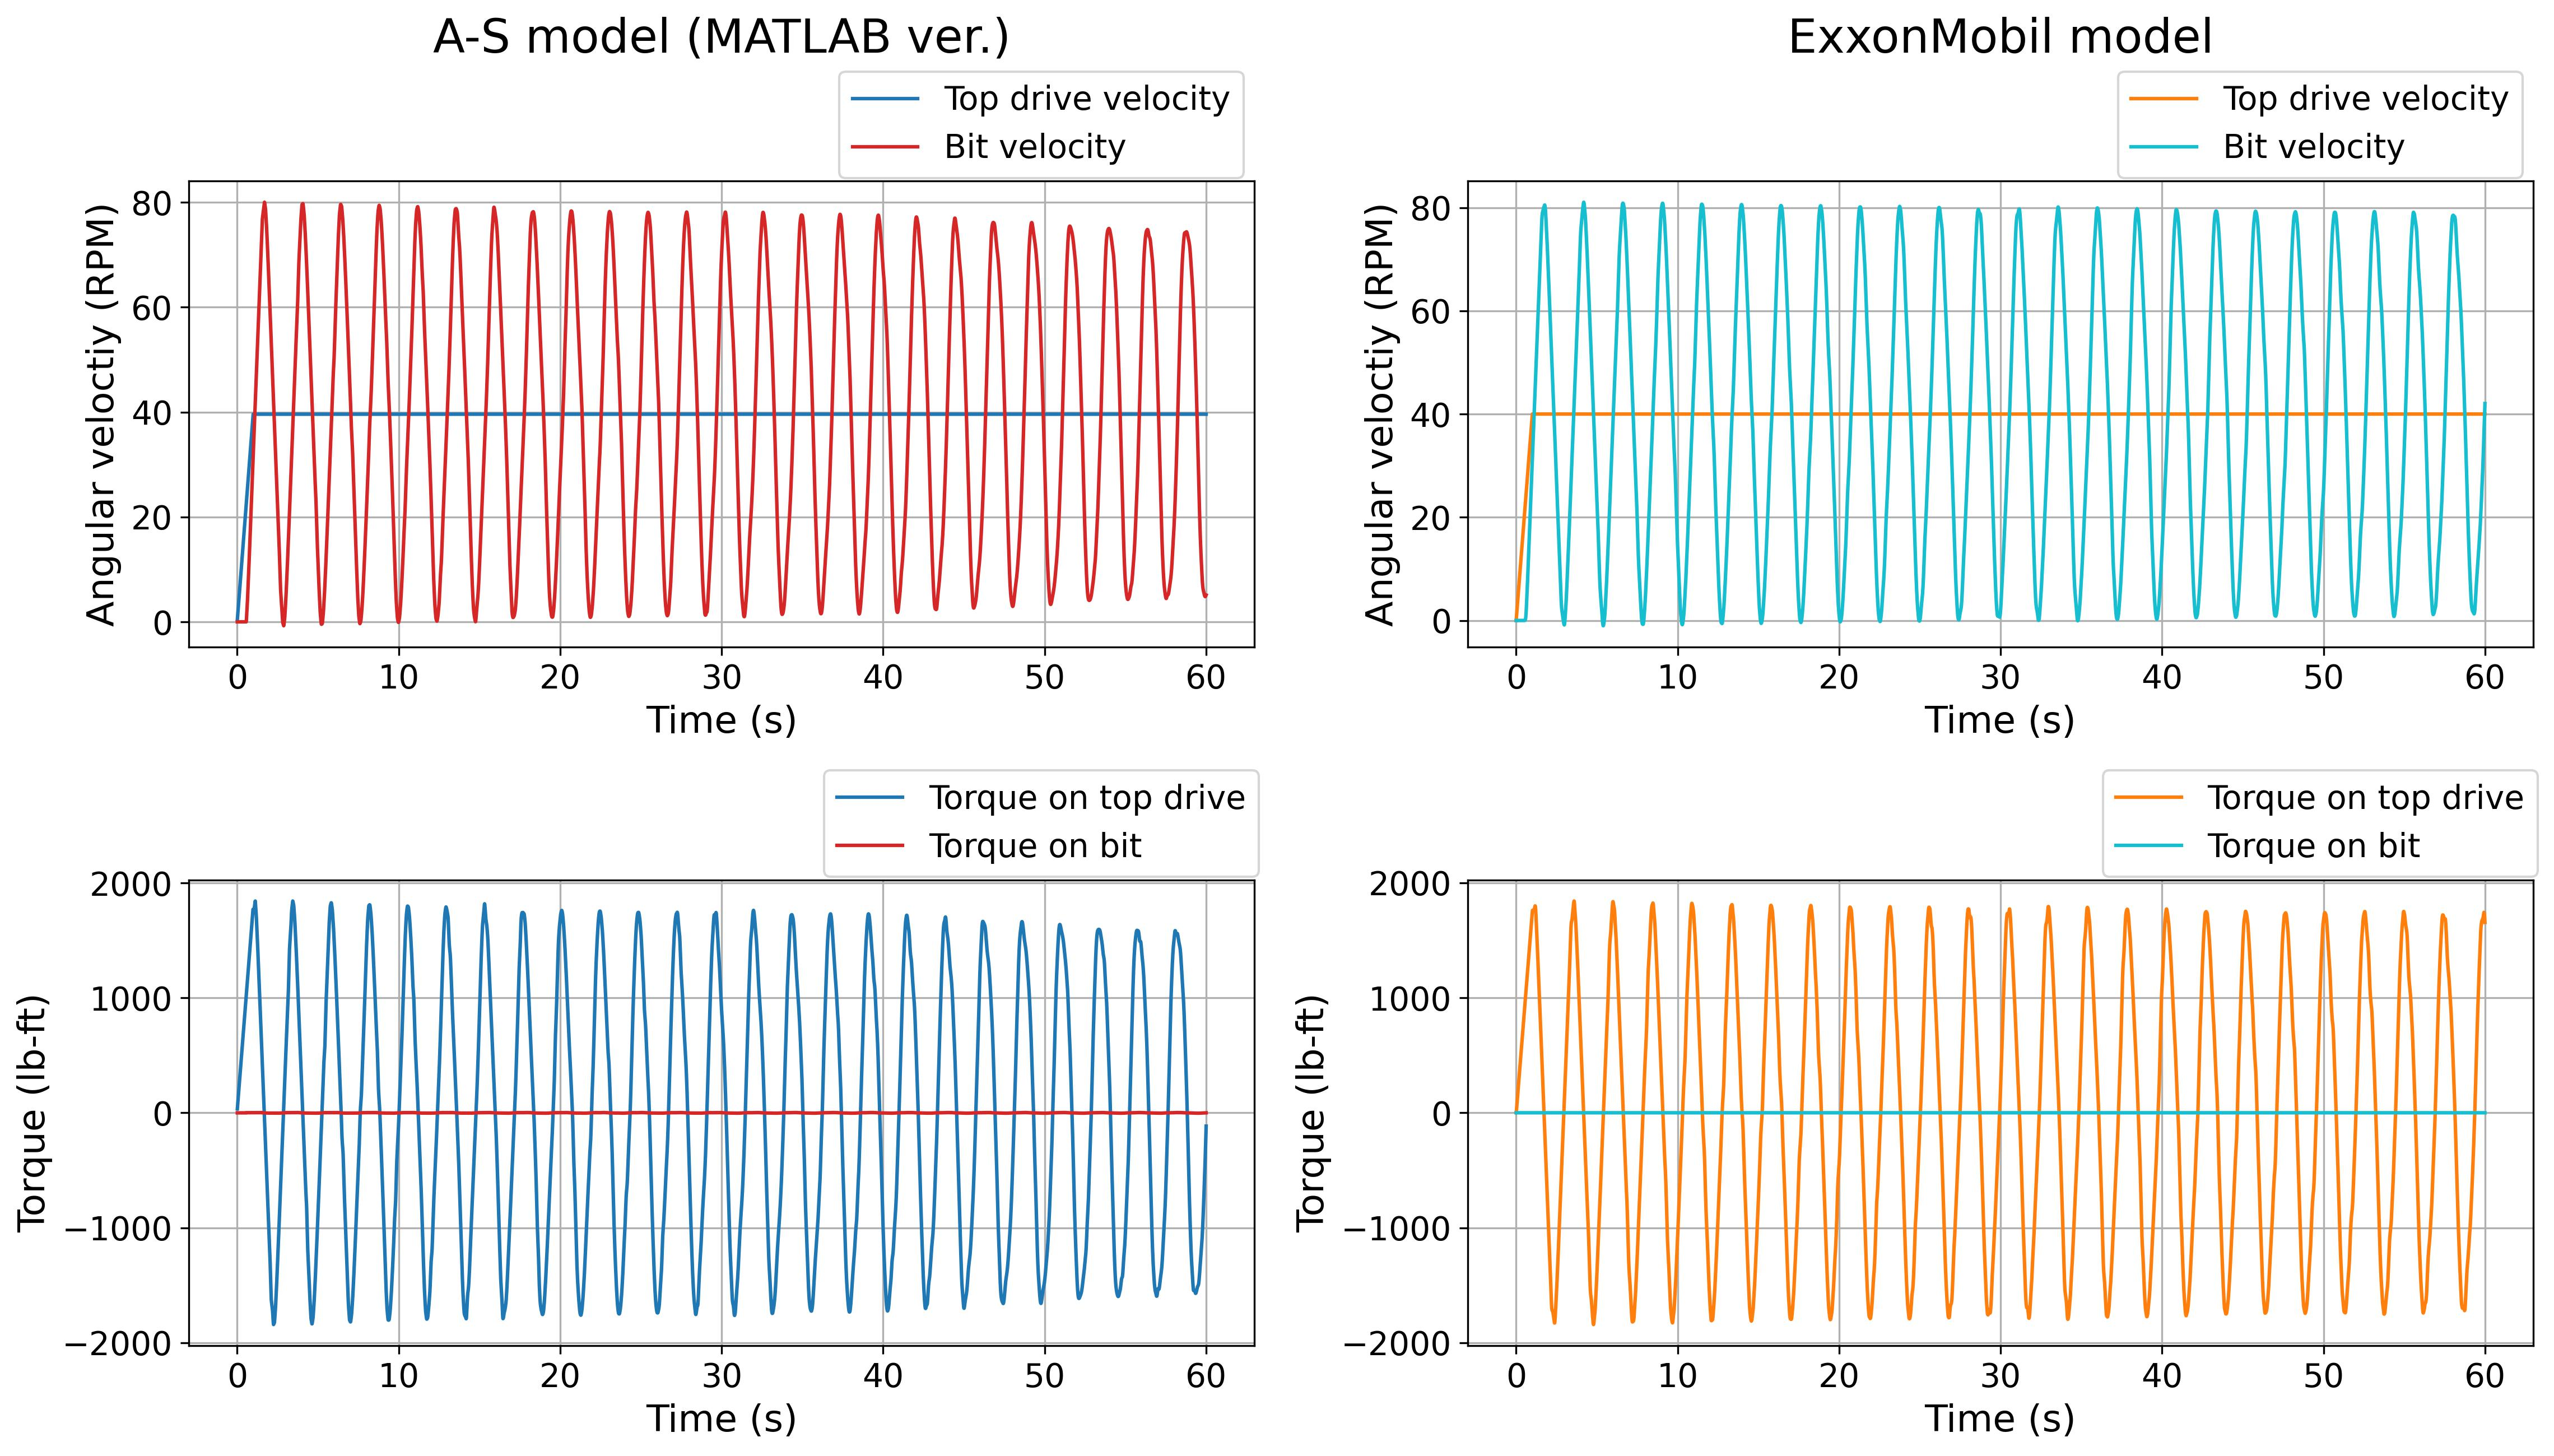
\includegraphics[width=6.5in]{output_figureTestCase3}
  \caption[Angular velocity and torque plots for Test Case 3]{Angular velocity and torque plots for Test Case 3. First and second columns show the results from the A-S model (Matlab ver.) and the ExxonMobil model, respectively.}\label{figure_testcase3}
\end{figure}
\begin{figure}
  \centering
  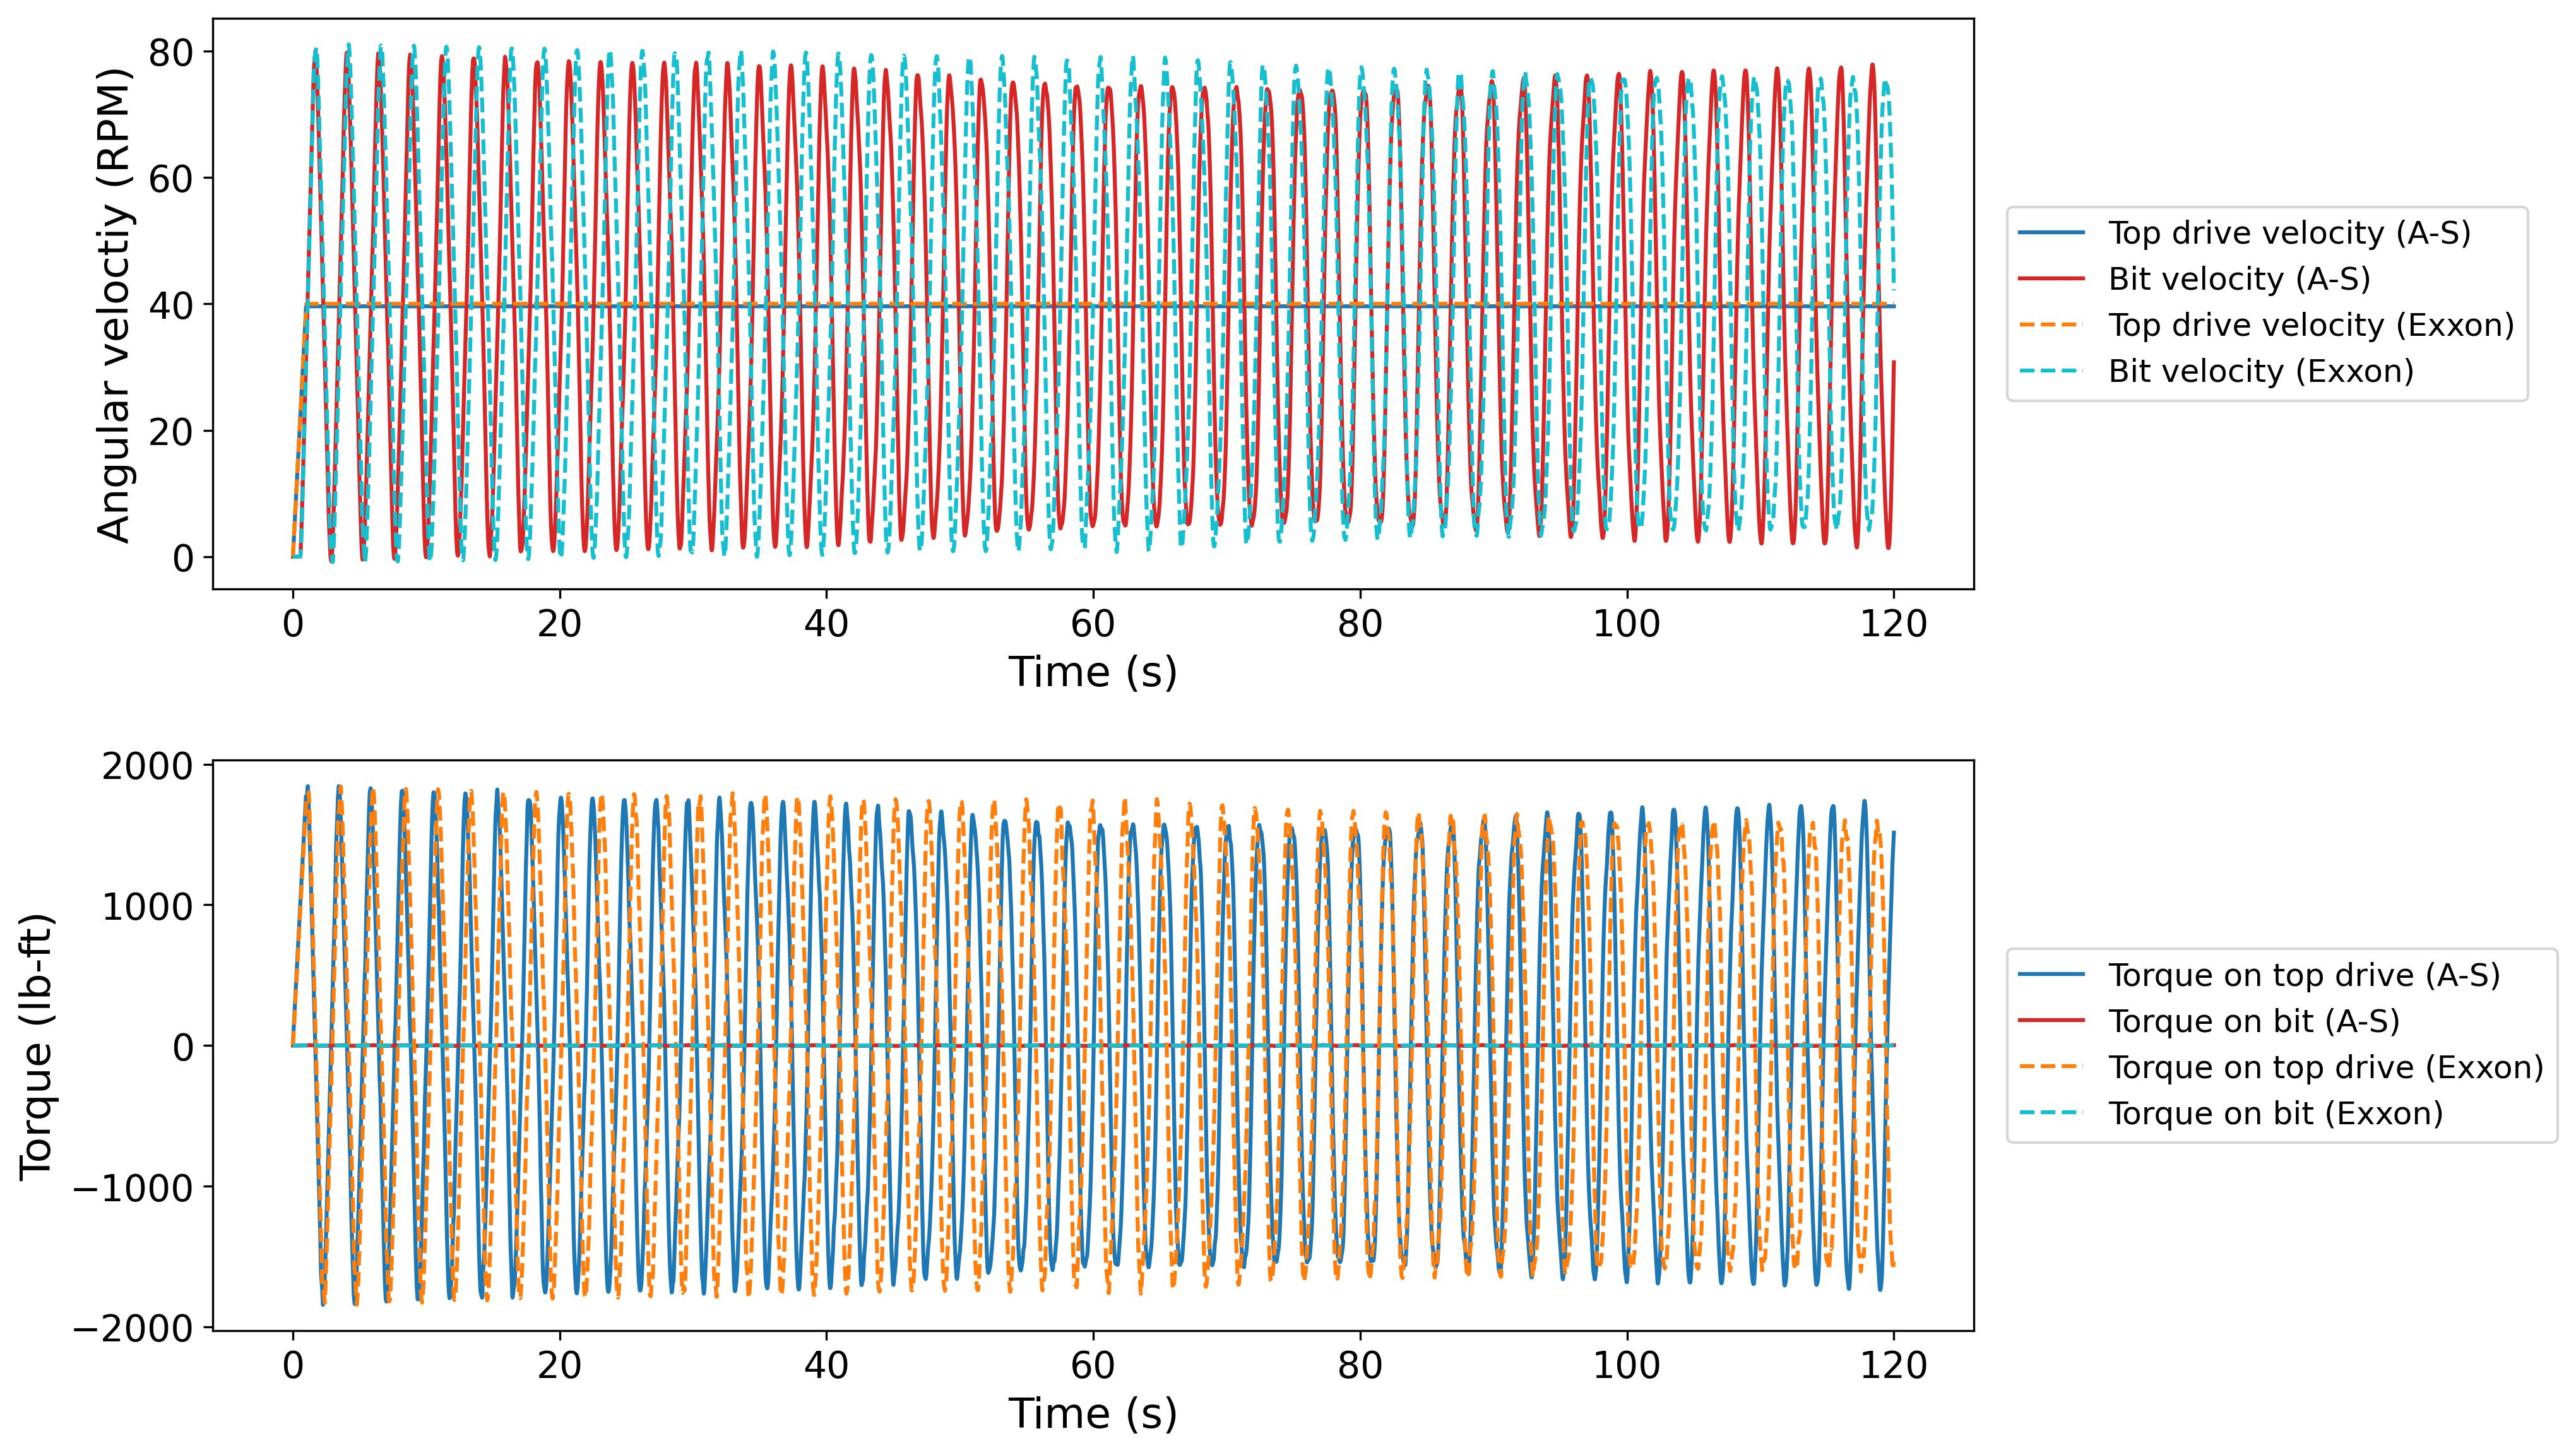
\includegraphics[width=6.5in]{overlapped_figureTestCase3_1}
  \caption[Angular velocity and torque comparison plots for Test Case 3]{Angular velocity and torque comparison between the results from the A-S model (Matlab ver.) and the ExxonMobil model for Test Case 3. The fundamental vibration frequencies are 0.420 $Hz$ from the A-S model and 0.408 $Hz$ from the ExxonMobil model. The difference in frequency is small, but the accumulated effect of these differences caused the phase shift during 60 seconds. Overall, both models matched well. Fluctuations in the amplitude of the bit angular velocity and the top drive torque are observed, which results from BHA components.}\label{figure_testcase3_overlapped}
\end{figure}

\begin{table}
\centering
\begin{tabular}{|c|c|c|}
\hline
\tablecolumnheadervlinesone{} & \tablecolumnheadervlinestwo{A-S Model} & \tablecolumnheadervlinestwo{ExxonMobil Model} \\
\hline
Frequency & 0.420 $Hz$ & 0.408 $Hz$\\
\hline
Maximum bit velocity & 80 $RPM$ & 81 $RPM$ \\
\hline
Maximum top drive torque & 1844 $lb\mbox{-}ft$ & 1841 $lb\mbox{-}ft$ \\
\hline
Computation time & 36 $s$ & 104 $s$\\
\hline
\end{tabular}
\caption[Comparison between the A-S and ExxonMobil models for Test Case 3]{Comparison between the A-S and ExxonMobil models for Test Case 3.}\label{table_summary_testcase3}
\end{table}

\section{Test Case 4}
Test Case 4 simulates a deviated well scenario with BHA components. In Test Case 4a, both the static and dynamic friction factors are set to 0.5 while Test Case 4b uses a static friction factor of 0.5 and a dynamic friction factor of 0.25.

\subsection{Test Case 4a}
Results for Test Case 4a for each model and the comparison between the two models are depicted in \figurename{}s~\ref{figure_testcase4_1} and~\ref{figure_testCase4_1_overlapped}, respectively. The features are summarized in \tablename~\ref{table_summary_testcase4a}. It can be seen that the effect of the BHA components are more significant in a deviated well as compared to a vertical well by comparing Test Cases 1 and 3 (vertical) with Test Cases 2a and 4a (deviated). The maximum top drive torque increased by about 1500 $lb\mbox{-}ft$ when adding the BHA components to the drill string, while the bit angular velocity was almost the same. The significant effect of \reviewcomment{increased what? Torque?}\resolvedcomment{} BHA components on top drive torque in deviated well  compared to vertical well can be the result of increased depth, increased friction. However, The shear modulus between Test Cases 2a,4a and Test Cases 1,3 are different and this difference in shear modulus might also affected the effect of BHA component in top drive torque \reviewcomment{How does shear modulus increase the torque?}\resolvedcomment{} (refer to input parameters in \chaptername~\ref{ch:testcases}). Additional sensitivity tests can be conducted to analyze the effect of BHA components on drill string vibration.

\begin{figure}
  \centering
  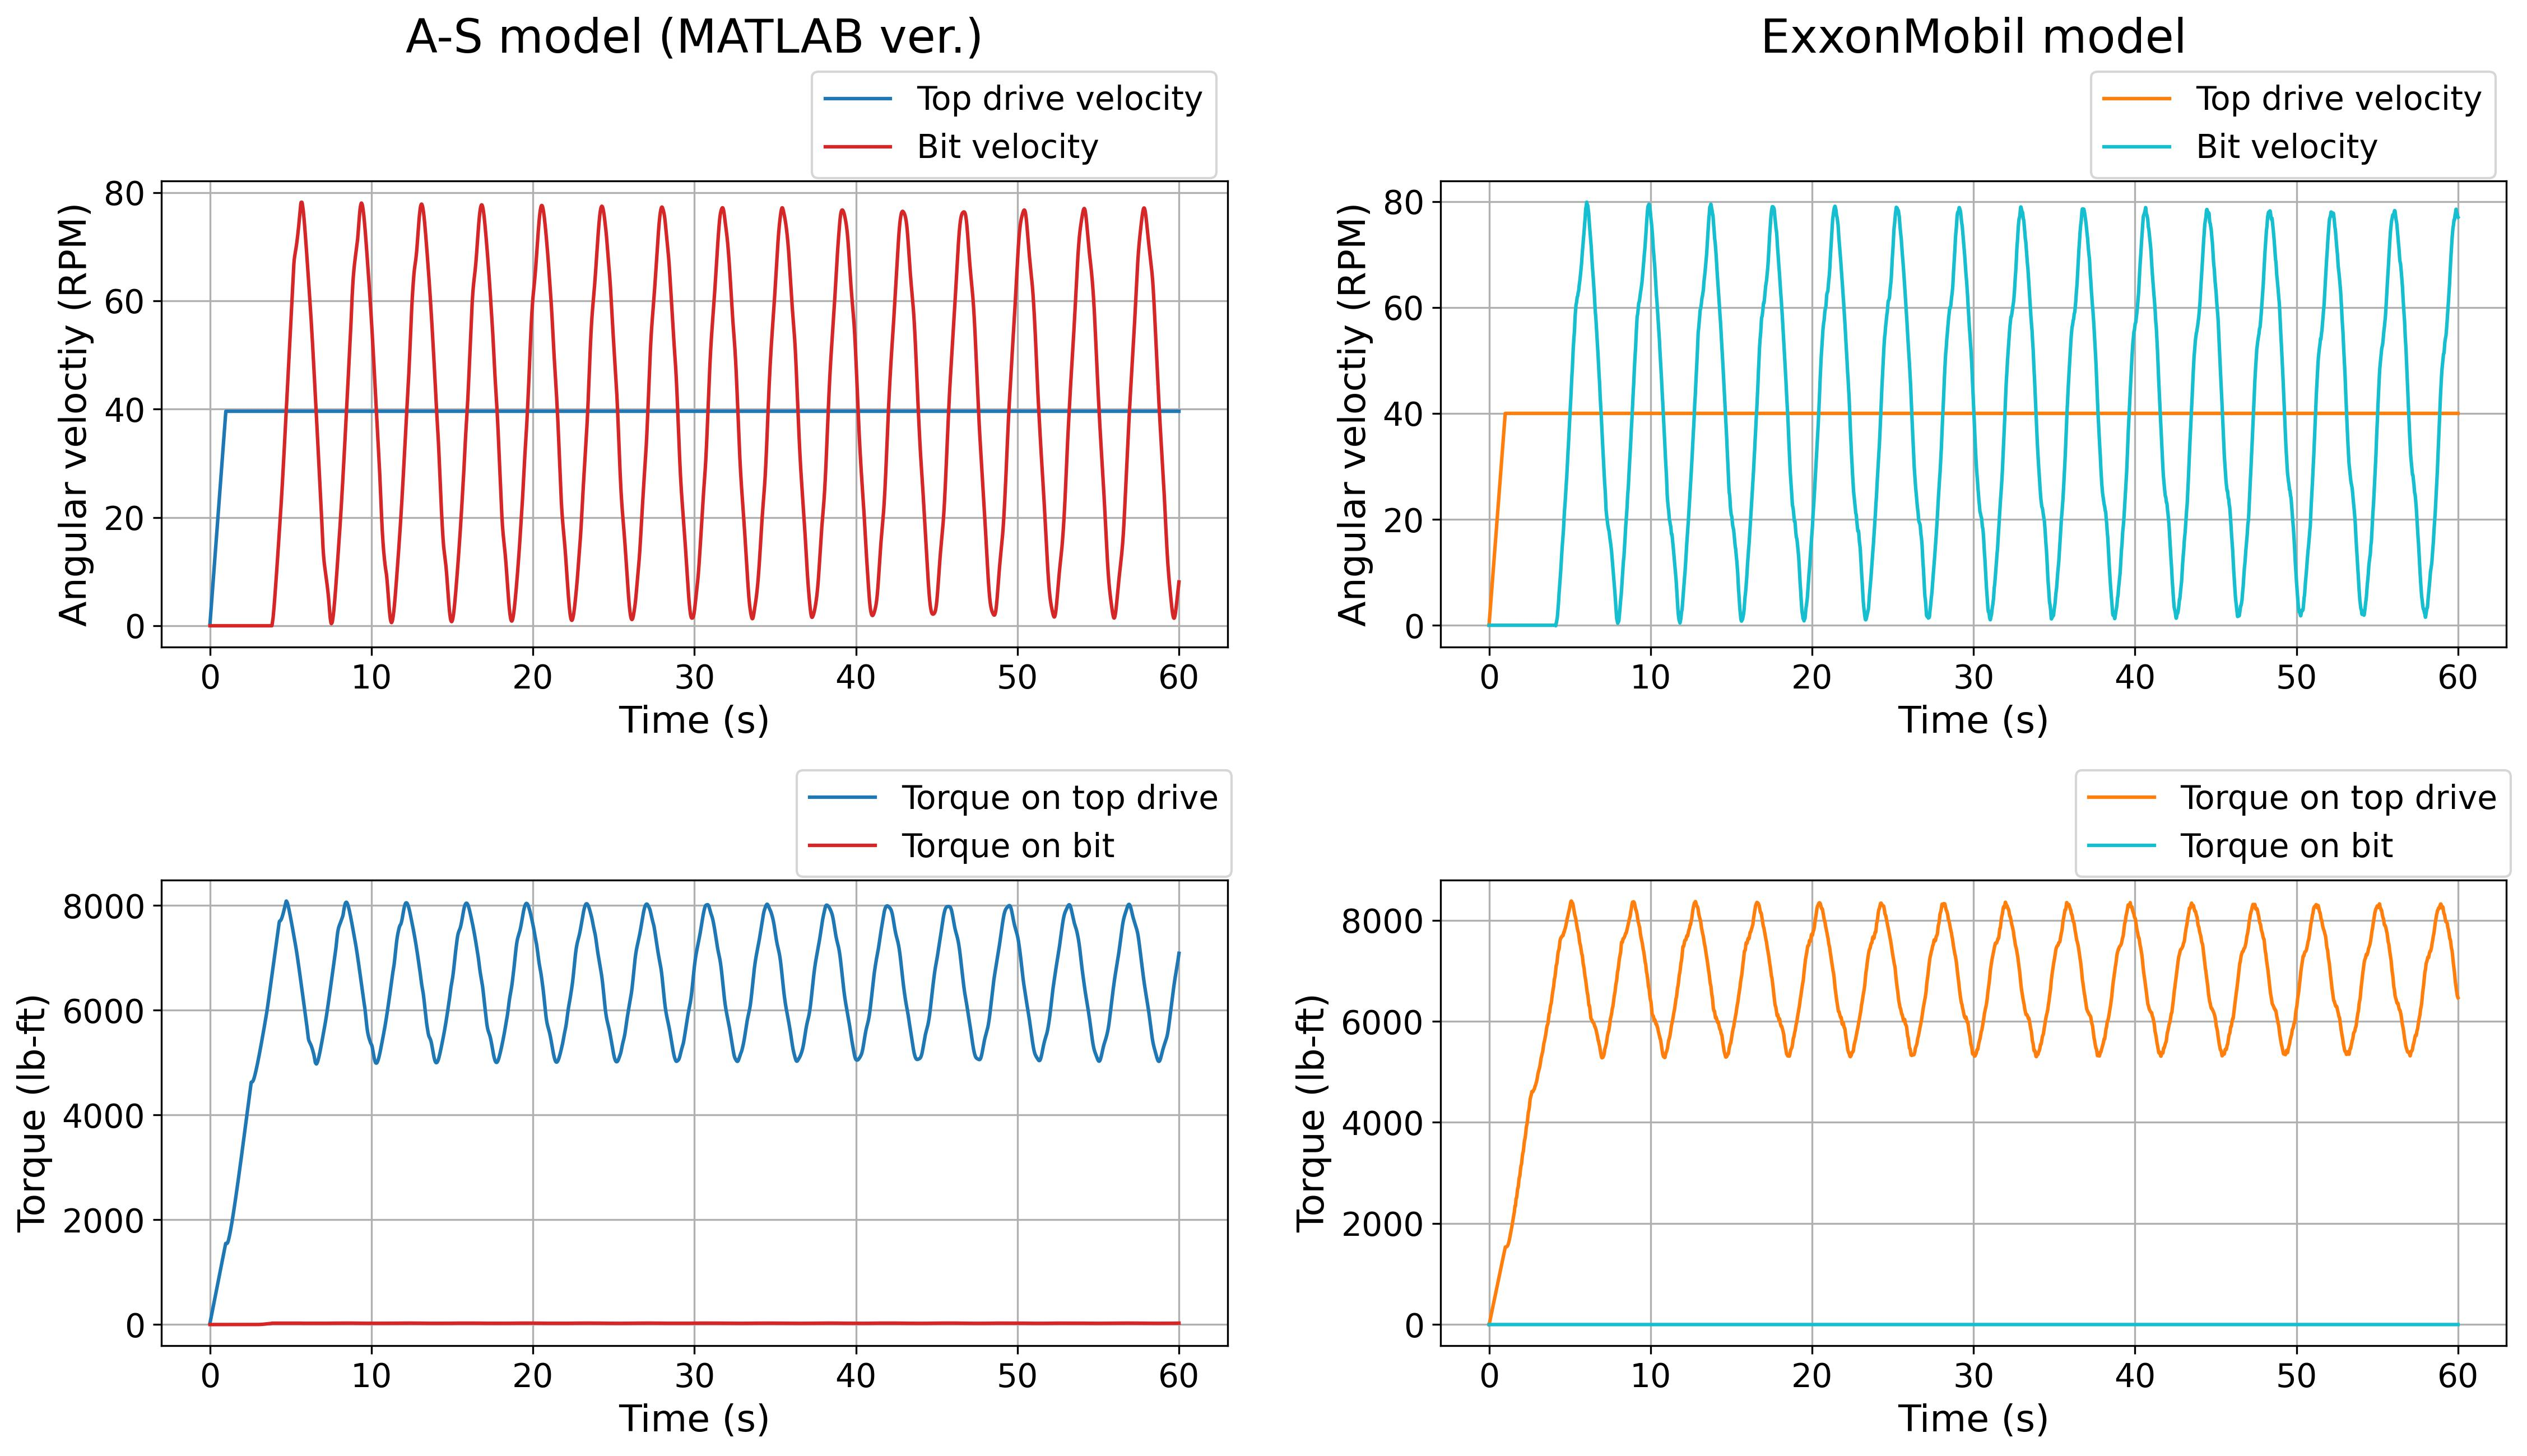
\includegraphics[width=6.5in]{output_figureTestCase4_1}
  \caption[Angular velocity and torque plots for Test Case 4a]{Angular velocity and torque plots for Test Case 4a. First and second columns show the results from the A-S model (Matlab ver.) and the ExxonMobil model, respectively.}\label{figure_testcase4_1}
\end{figure}

\begin{figure}
  \centering
  \includegraphics[width=6.5in]{overlapped_figureTestcase4_1}
  \caption[Angular velocity and torque comparison plots for Test Case 4a]{Angular velocity and torque comparison between the results from the A-S model (Matlab ver.) and the ExxonMobil model for Test Case 4a. The fundamental vibration frequency are 0.268 $Hz$ from the A-S model and 0.260 $Hz$ from the ExxonMobil model. The difference in frequency is small, but the accumulated effect of these differences caused the phase shift during 60 seconds. Overall, both models matched well.}\label{figure_testCase4_1_overlapped}
\end{figure}

\begin{table}
\centering
\begin{tabular}{|c|c|c|}
\hline
\tablecolumnheadervlinesone{} & \tablecolumnheadervlinestwo{A-S Model} & \tablecolumnheadervlinestwo{ExxonMobil Model} \\
\hline
Frequency & 0.268 $Hz$ & 0.260 $Hz$\\
\hline
Maximum bit velocity & 78 $RPM$ & 79 $RPM$ \\
\hline
Maximum top drive torque & 8083 $lb\mbox{-}ft$ & 8379 $lb\mbox{-}ft$ \\
\hline
Computation time & 32 $s$ & 231 $s$\\
\hline
\end{tabular}
\caption[Comparison between the A-S and ExxonMobil models for Test Case 4a]{Comparison between the A-S and ExxonMobil models for Test Case 4a.}\label{table_summary_testcase4a}
\end{table}

\subsection{Test Case 4b}
The comparison between the A-S and ExxonMobil models are illustrated in \figurename~\ref{figure_testcase4_2_overlapped} and the features are summarized in \tablename~\ref{table_summary_testcase4b}.
Except the shift in the phase that gradually occurred over the 60 seconds modeled, both models matched in overall behavior. They both demonstrated stick-slip with similar characteristics.

The effect of BHA components in deviated well is more detailed in \figurename{}s~\ref{figure_BHA_Matlab} and~\ref{figure_BHA_EXXON} from the A-S and the ExxonMobil model, respectively. Adding the BHA slowed down the vibration while increased the torque on top drive. Specifically, the spikes on top drive were observed in both models before the stick phase. These sudden spikes were more significant in the A-S model.


\begin{figure}
  \centering
  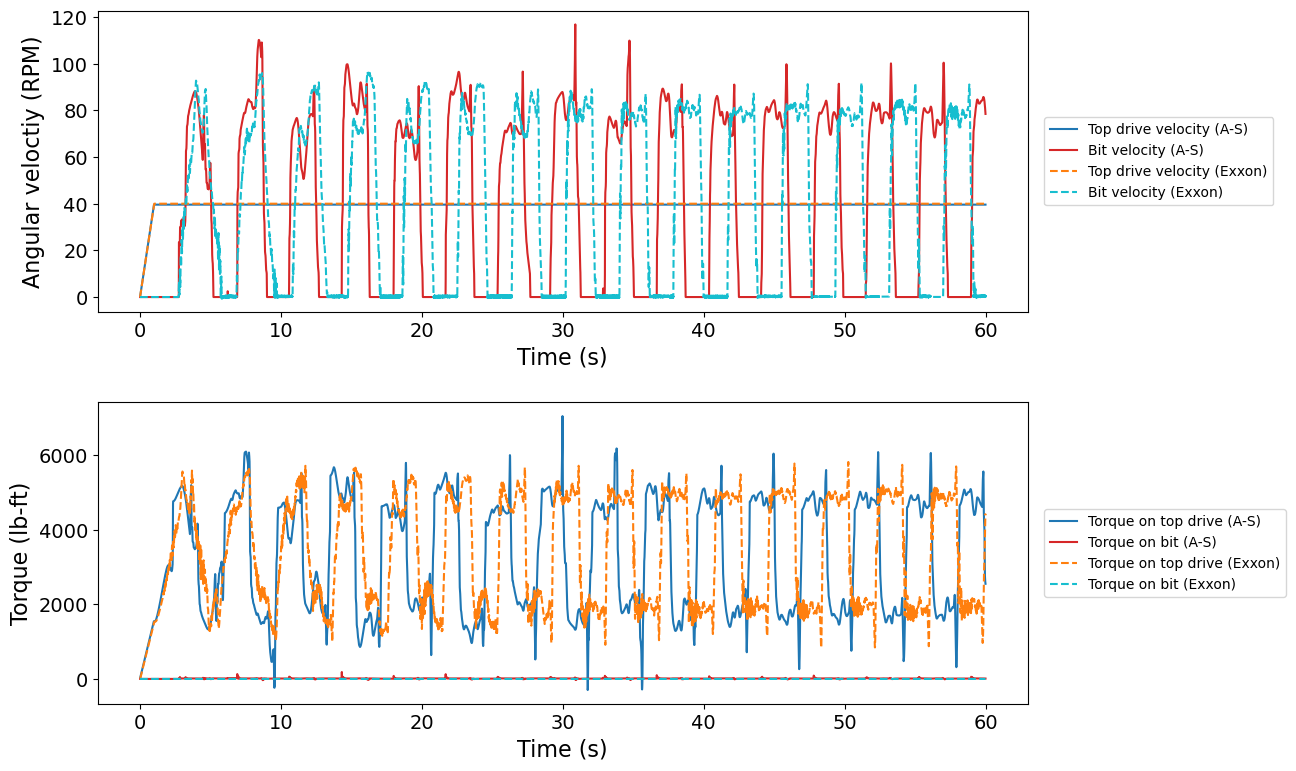
\includegraphics[width=6.5in]{overlapped_figureTestCase4_2}
  \caption[Angular velocity and torque comparison plots for Test Case 4b]{Angular velocity and torque comparison between the results from the A-S model (Matlab ver.) and the ExxonMobil model for Test Case 4b. The fundamental vibration frequency are 0.268 $Hz$ from the A-S model and 0.260 $Hz$ from the ExxonMobil model. The difference in frequency is small, but the accumulated effect of these differences caused the phase shift during 60 seconds. Overall, both models matched well. Even the transient phase (before 40 seconds) showed similar vibration patterns for both models. Both models predicted a similar standstill for about 1.6-1.7 seconds during stick state in steady phase (after 40 seconds). The spikes in bit angular velocity and torque on top drive were observed from both models, which was not observed when there was no BHA. The amount of spike is more significant in A-S model compared to ExxonMobil model.}\label{figure_testcase4_2_overlapped}
\end{figure}

\begin{table}
\centering
\begin{tabular}{|c|c|c|}
\hline
\tablecolumnheadervlinesone{} & \tablecolumnheadervlinestwo{A-S Model} & \tablecolumnheadervlinestwo{ExxonMobil Model} \\
\hline
Frequency & 0.268 $Hz$ & 0.260 $Hz$\\
\hline
Maximum bit velocity & 116 $RPM$ & 96 $RPM$ \\
\hline
Maximum top drive torque & 7056 $lb\mbox{-}ft$ & 5825 $lb\mbox{-}ft$ \\
\hline
Computation time & 32 $s$ & 231 $s$\\
\hline
\end{tabular}
\caption[Comparison between the A-S and ExxonMobil models for Test Case 4b]{Comparison between the A-S and ExxonMobil models for Test Case 4b.}\label{table_summary_testcase4b}
\end{table}


\begin{figure}
  \centering
  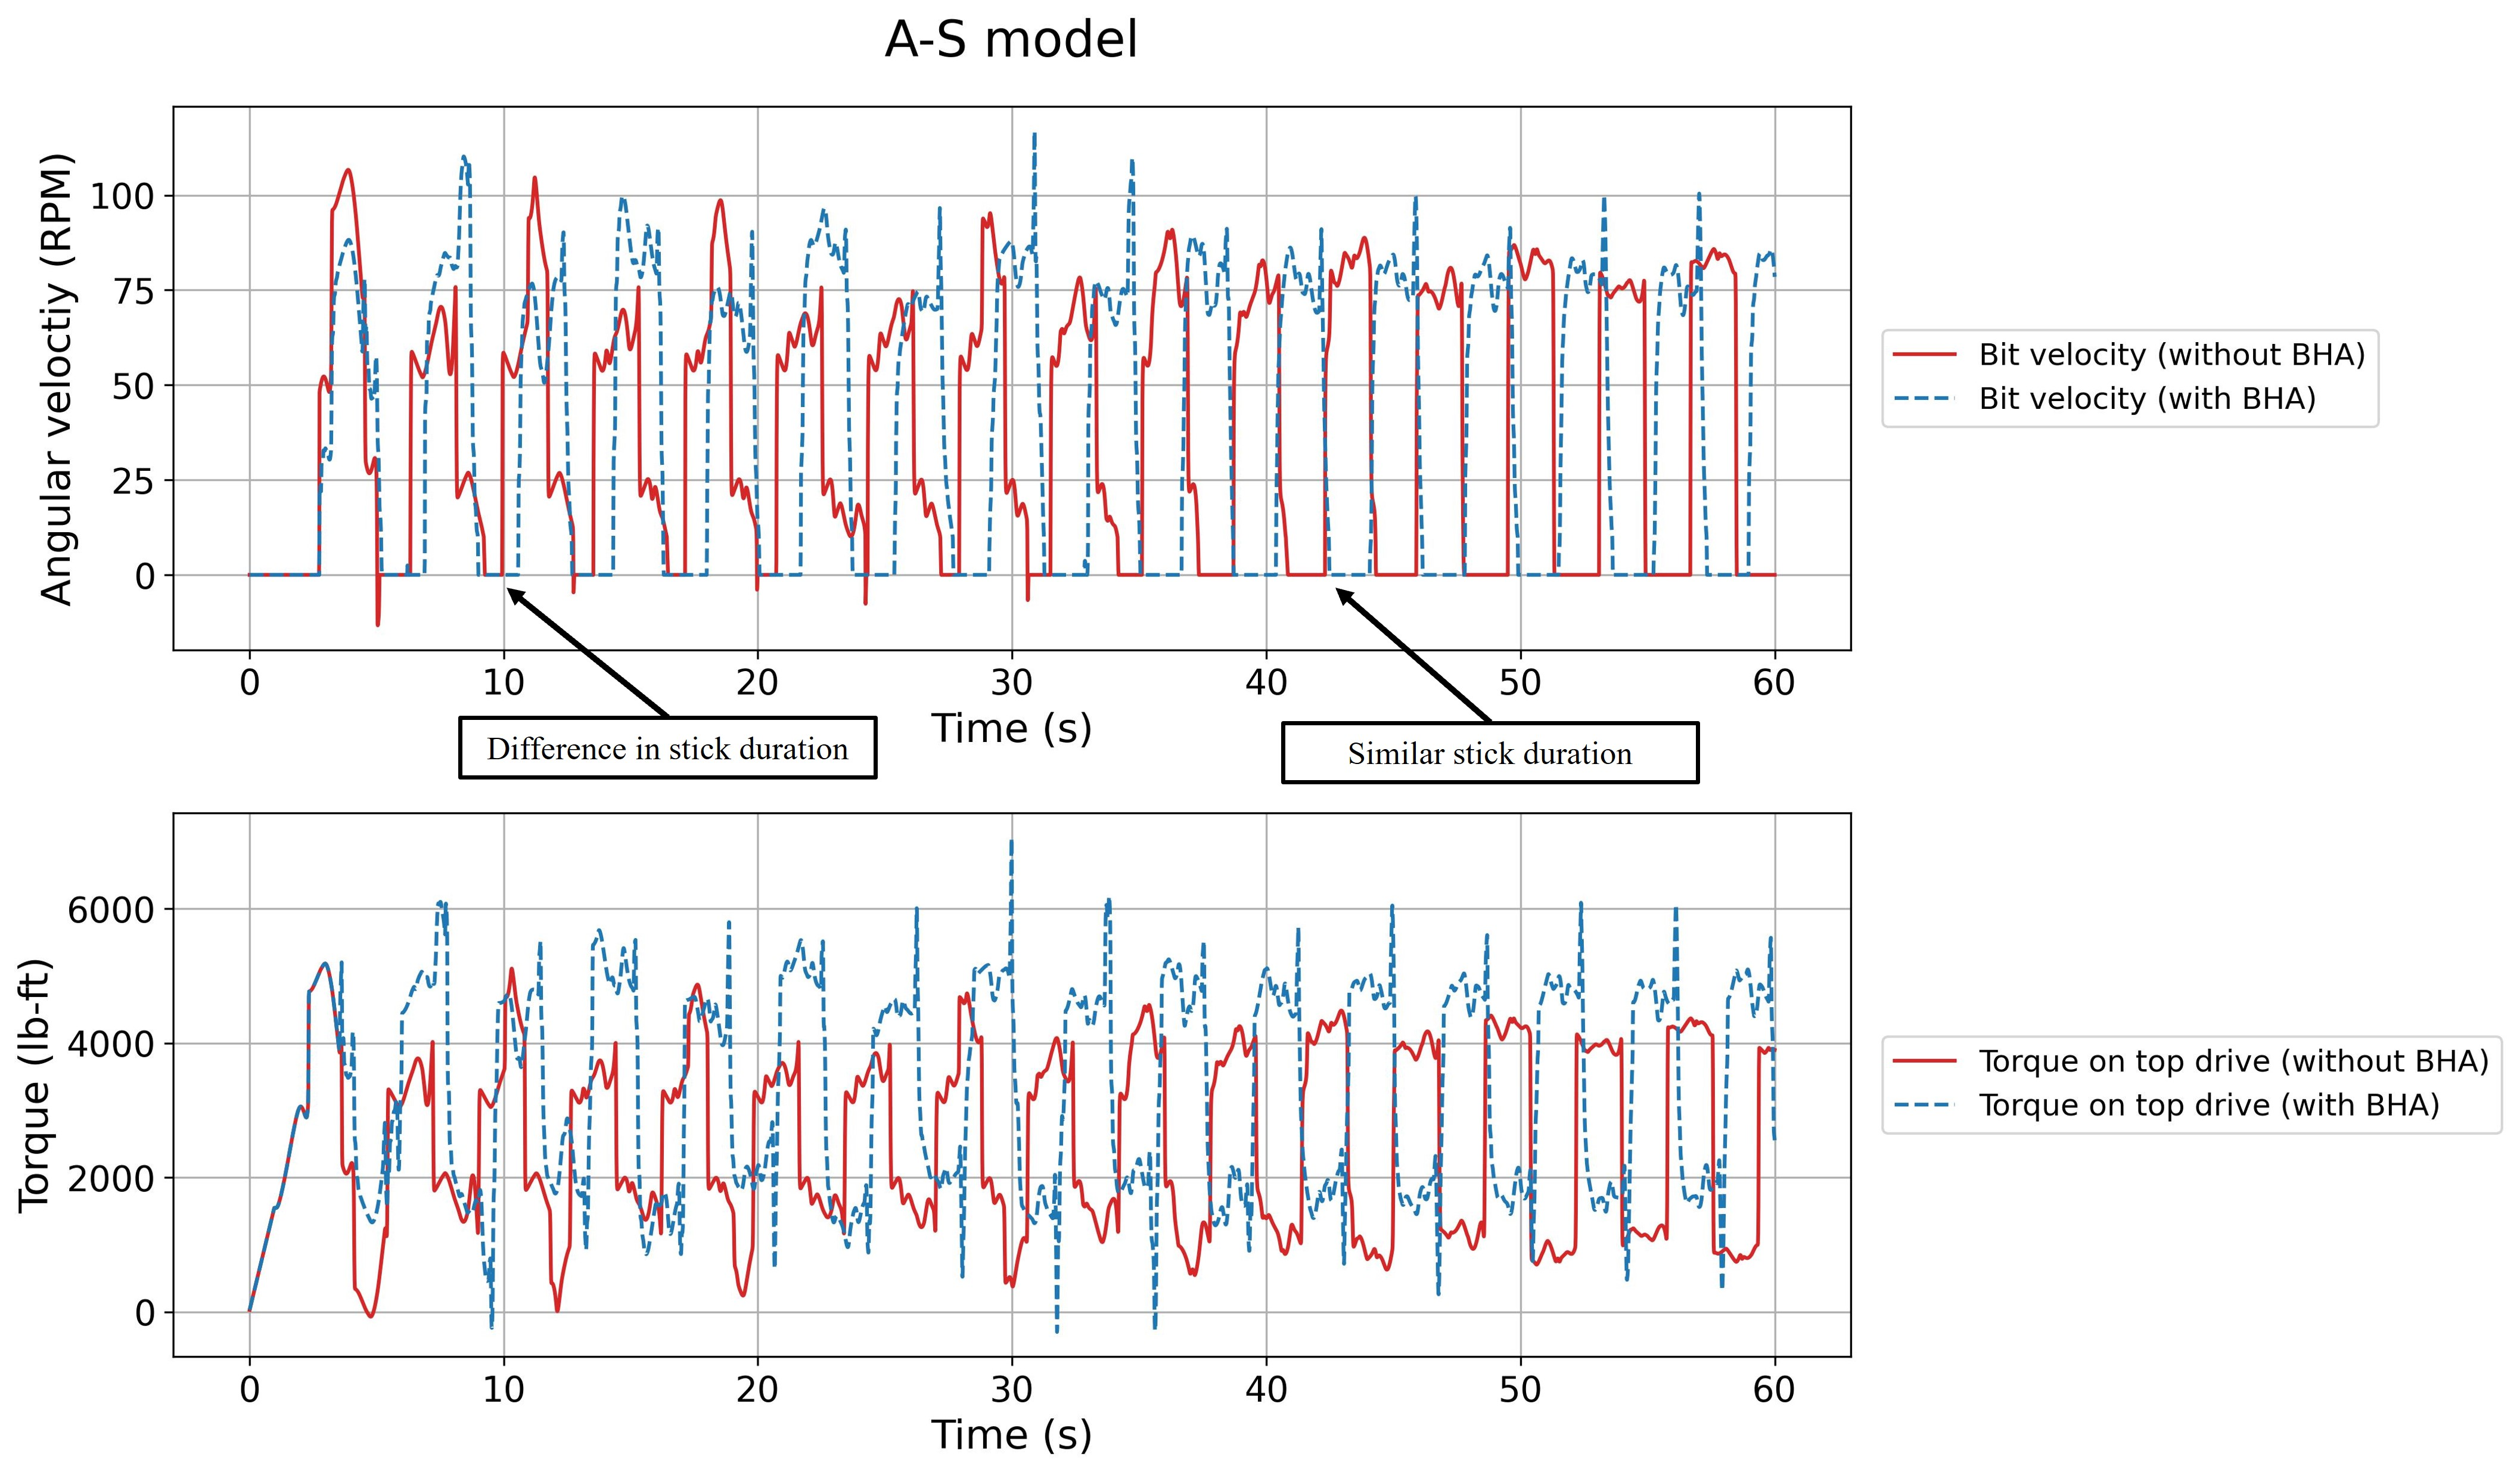
\includegraphics[width=\linewidth]{BHA_ml_arrow}
  \caption[Effects of BHA components in a deviated well from the A-S model]{A comparison of the effects of BHA components in a deviated well as predicted by the A-S model. The graph shows the comparison between Test Case 2b and 4b. Adding BHA components increased the torque on top drive. Spikes in the maximum torque and bit velocity are observed when a BHA is added. Spikes below 0 $RPM$ in the bit velocity are only observed when there are no BHA components. With a BHA, the stick phase of the initial 2-3 cycles is longer; however, later in the simulation the length of the stick phase is similar (about 1.6-1.8 seconds). The fundamental frequency of the vibration decreases when a BHA exists.}\label{figure_BHA_Matlab}
\end{figure}

\begin{figure}
  \centering
  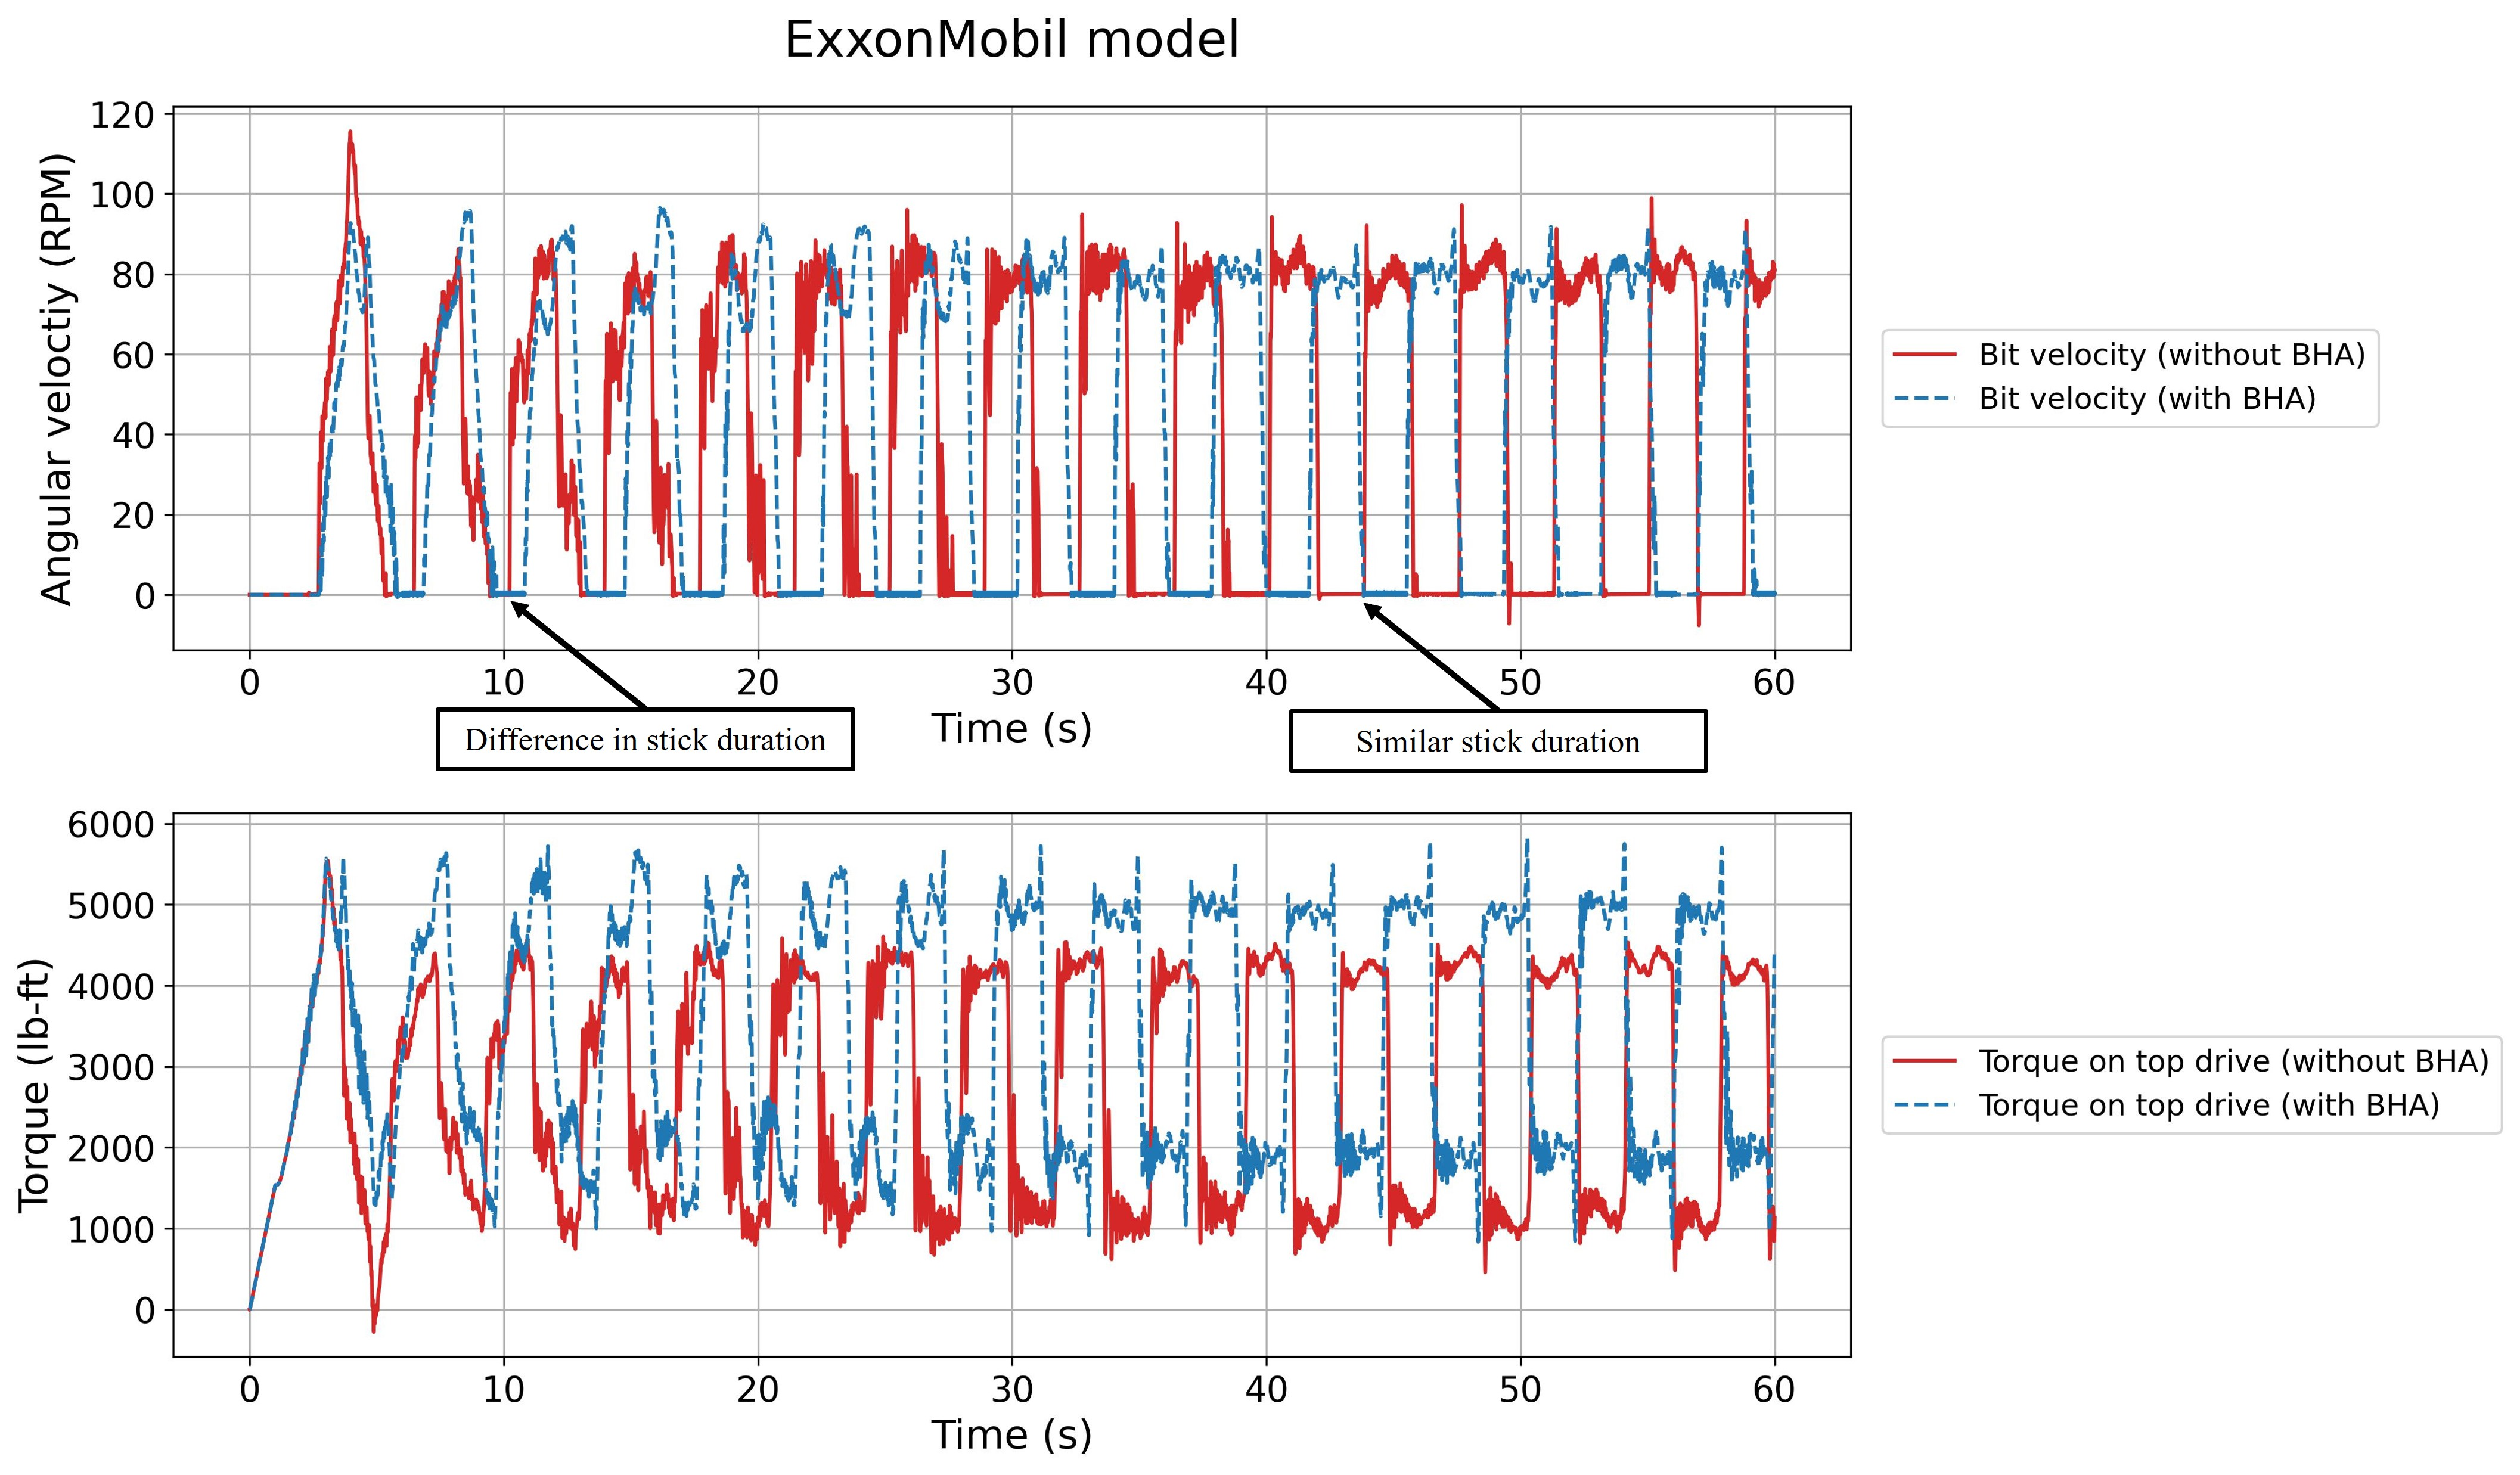
\includegraphics[width=\linewidth]{BHA_exxon_arrow}
  \caption[Effects of BHA components in a deviated well from the ExxonMobil model]{A comparison of the effects of BHA components in a deviated well as predicted by the ExxonMobil model. The graph shows the comparison between Test Case 2b and 4b. Adding BHA components increased the torque on top drive. Spikes in the maximum torque and bit velocity are observed when a BHA is added. Spikes below 0 $RPM$ in the bit velocity are only observed when there are no BHA components. With a BHA, the stick phase of the initial 2-3 cycles is longer; however, later in the simulation the length of the stick phase is similar (about 1.6-1.8 seconds). The fundamental frequency of the vibration decreases when BHA exists.}\label{figure_BHA_EXXON}
\end{figure}

\section{Summary and Observations}
The results from the A-S model and ExxonMobil model for all the Test Cases are summarized in \tablename{}s~\ref{AS_results_summary} and~\ref{Exxon_results_summary}, respectively. Overall, both models showed comparable predictions across all the Test Cases. Additionally, the run times of the simulations are included in the table.  The simulations were conducted with a computing system featuring Intel\textsuperscript{\textregistered} Core\textsuperscript{\texttrademark} i7-8650U CPU and 16GB RAM\@.

\begin{table}
    \centering
	\begin{testcaseresulttable}
        Test Case 1 & 0.440 & 1762 & 79 & 36\\
        \hline
        Test Case 2a & 0.283 & 6643 & 78 & 25\\
        \hline
        Test Case 2b & 0.280 & 5184 & 106 & 25\\
        \hline
        Test Case 3 & 0.420 & 1844 & 80 & 36\\
        \hline
        Test Case 4a & 0.268 & 8083 & 78 & 32\\
        \hline
        Test Case 4b & 0.268 & 7056 & 116 & 32\\
        \hline
    \end{testcaseresulttable}
    \caption[Summary of simulation results for A-S model]{Summary of simulation results for A-S model.} \label{AS_results_summary}
\end{table}

\begin{table}
    \centering
	\begin{testcaseresulttable}
        Test Case 1  & 0.427 & 1814 & 81 & 106\\
        \hline
        Test Case 2a  & 0.272 & 6891 & 79 & 117\\
        \hline
        Test Case 2b  & 0.269 & 5539 & 115 & 116\\
        \hline
        Test Case 3  & 0.408 & 1841 & 81 & 104\\
        \hline
        Test Case 4a  & 0.260 & 8379 & 79 & 231\\
        \hline
        Test Case 4b & 0.260 & 5825 & 96 & 231\\
        \hline
    \end{testcaseresulttable}
    \caption[Summary of simulation results for ExxonMobil model]{Summary of simulation results for ExxonMobil model.}
    \label{Exxon_results_summary}
\end{table}

Some of the key observations are listed below.
\begin{bulletedlist}
    \item The models matched well in both the transient and steady-state sections.
    \item Adding BHA components caused larger fluctuations in the peak values of the top drive torque and bit angular velocity in a vertical well.
    \item Spike in top drive torque is observed before the stick phase only when the BHA components were added to the drill string, which was more significant in A-S model. \reviewcomment{This is hard to understand.}
    \item Spikes in the bit angular velocity with negative values were observed before the stick phase when the simulation was ran without BHA components. \reviewcomment{Before the stick phase?  At the start of the stick phase?}
    \item The A-S model was able to run faster than real time, a feature attributed to the flexibility in time step
    \item The ExxonMobil model exhibited small movements in the bit position in the stick phase
\end{bulletedlist} 